%%%%%%%%%%%%%%%%%%%%%%%%%%%%%%%%%%%%%%%%%%%%%%%%%%%%%%%%%%%%%%%
\section{Production and Assembly}
\label{sec:fdsp-pd-prod-assy}
%\metainfo{(Length: TDR=40 pages, TP=8 pages)}

%%%%PHOTON COLLECTORS PRODUCTION %%%%%%%%%%%%%%%%%%%%%%%%%%%%%%%%%%%%%%%%%%%%%%%%%%%

\subsection{Photon Collector Production}
\label{sec:fdsp-pd-prod-pc}
%\metainfo{\color{blue} Content: Cavanna/Whittington/Machado}

In this section we will first describe the production process specific to each of the three Photon Collector technologies, followed by the final assembly procedures common to all types. 

%%%%ARAPUCA %%%%%%%%

\subsubsection{ARAPUCA}
\label{ssec:fdsp-pd-pc-prod-arapuca}
%\fixme{This section remains to be updated.}
% New from Ana added 8 apr 18
Although the individual cell dimensions may differ, the basic design of the ARAPUCA-based photon detector modules for the first module of the Single-Phase DUNE far detector will be similar to that of the two prototypes produced for ProtoDUNE-SP. Here we describe the production and assembly envisaged based on that experience.

Each ProtoDUNE-SP ARAPUCA module is shaped as a bar with external dimensions of 
\SI{207.3}{cm}$ \times$ \SI{9.6}{cm} $\times$ \SI{1.46}{cm}, which allows for it to be inserted between the wire planes through 10 slots the APA. The module currently contains sixteen basic ARAPUCA cells, each one with an optical window with an area of \SI{7.8}{cm} $\times$ \SI{9.8}{cm} and internal dimensions of approximately \SI{8}{cm} $\times$ \SI{10}{cm} $\times$ \SI{0.6}{cm}. The SiPMs are mounted on the backplane of the cell, which in ProtoDUNE-SP, allows for  two different configurations of either 12 or 6 passively-ganged SiPMs.

%(Picture 1)
\begin{dunefigure}[ProtoDUNE-SP ARAPUCA modules during assembly.]{fig:arap-prod01}
{ProtoDUNE-SP ARAPUCA modules during assembly prior to installation of the dichroic filters; SiPMs and TPB coated reflector are visible.}
  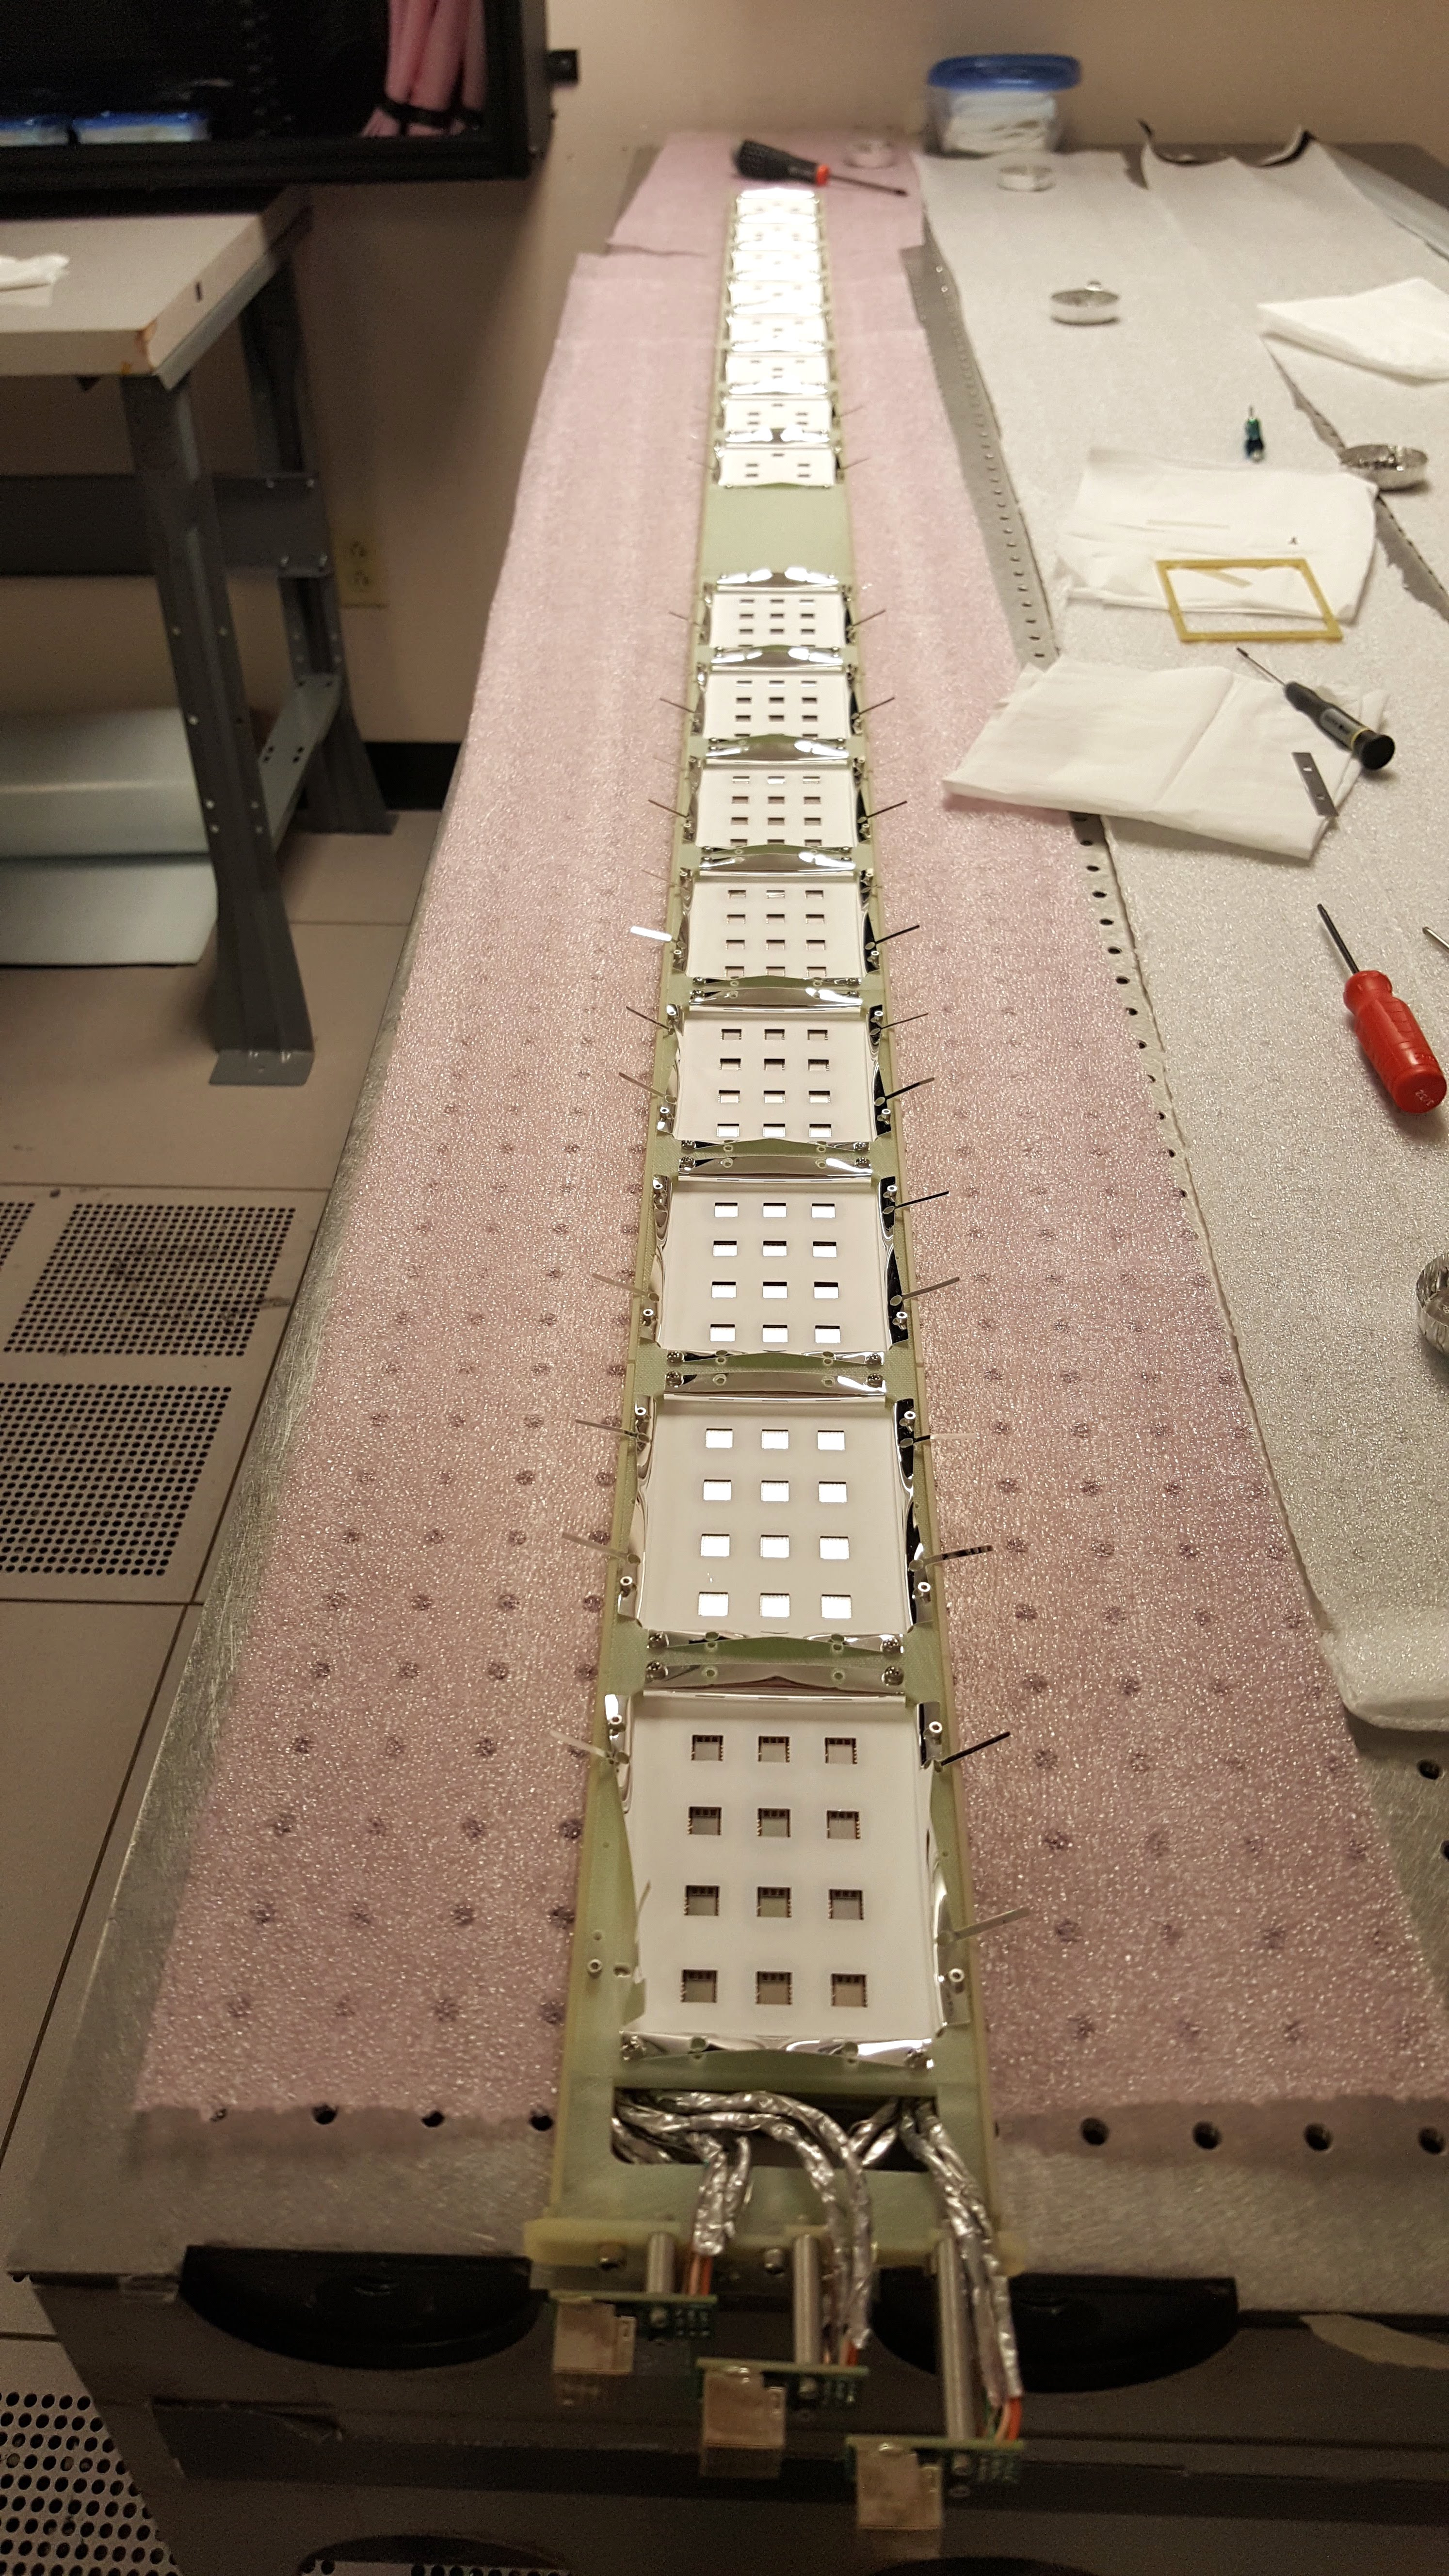
\includegraphics[height=8cm]{pds-arapuca-protodune02-apr18}
\end{dunefigure}

The internal surface of the box is lined with a dielectric mirror foil\footnote{3M Vikuiti\texttrademark\  ESR - http://multimedia.3m.com/mws/media/193294O/vikuiti-tm-esr-application-guidelines.pdf} laser cut with openings at the locations of the SiPMs; these are visible in Figure~\ref{fig:arap-prod01}, which shows an ARAPUCA during assembly prior to installation of the optical windows. The backplane SiPM boards for the ProtoDUNE-SP modules were designed at CSU and produced by an external vendor\footnote{Advanced Circuits Inc.; www.4pcb.com.}; the SiPMs were soldered on the boards using a reflow oven at CSU. Before mounting into the ARAPUCA module they were tested at room and LN2 temperatures. It is anticiapted that the production of the boards for DUNE far detector will move to Brazil.
 %and the design will be optimized by Latin American institutions in collaboration with CSU.

The optical window of each box is a dichroic filter with cut-off at \SI{400}{nm}. While the filters used for the ProtoDUNE-SP prototypes have been acquired from Omega Optical Inc.\footnote{http://www.omegafilters.com/}, other vendors are being considered for the DUNE production\footnote{ASHAI -Japan, Andover-USA, Edmunds Optics-USA}.
Prior to coating, the filters are cleaned according to the procedures given by the manufacturer using isopropyl alcohol. Since the most likely vector for scratching/damaging the coating is dragging contaminated wipes across the surface, new clean lint free wipes are used for each  cleaning pass on the surface. Clean filters are then baked at 100$^\circ$C for \SI{12}{hours}. The Vikuiti\texttrademark\  foils do not need to be cleaned and baked since they have a protective film that is removed just before the evaporation.
   
The filters are coated on the external side facing the LAr active volume with pTP,
%para-Therphenyl, 
while the internal dielectric mirror side is coated with TPB.
%TetraPhenyl-Butadiene. 
The coatings for the ProtoDUNE-SP modules have been made at the Thin Film facility at Fermilab using a vacuum evaporator. Each coated filter was dipped in LN2 to check the stability of the evaporated coating at cryogenic temperature. For SPFD PD production the evaporation process will be performed at UNICAMP in Brazil, where a large vacuum evaporator with an internal diameter of one meter is now available. The  conversion efficiency of the film deposited on the filters or on the Vikuiti\texttrademark\   foils will be measured with a dedicated set-up that will use the \SI{128}{nm} light produced by a VUV monochromator.


%(Picture 2)


%%===Old pre-08apr ARAPUCA Prod text below ======================== 
%Each ARAPUCA module is composed of the following elements: 
%\begin{itemize}
%\item Dichroic filters coated with pTP 
%\item backplane board where the SiPMs are soldered and ganged together passively or actively
%\item reflective film to line the internal surface coated with TPB 
%\item mechanical frames  
%\end{itemize}

%The filters will be acquired from vendors who specialize in high-quality optical components. A number of vendors are currently being considered: ASHAI (Japan), Omega (US), Andover (US), Edmunds Optics (US). The coating of the filters will be performed in Brazil at the LAr facility at UNICAMP.  

%The reflective film is 3M Vikuiti ESR (http://multimedia.3m.com/mws/media/193294O/Vikuiti-tm-esr-application-guidelines.pdf), which will be coated with a thin layer of TPB by vacuum evaporation at the LAr facility of UNICAMP.  

%The quality of the evaporations on both the filters and the reflective foils will be tested in a dedicated facility (developed by and located at UNICAMP) where they will be irradiated with a pulsed VUV light and the response detected by photomultipliers.   

%The backplane board will be fabricated in Brazil by a commercial vendor yet to be selected, and the SiPMs will be soldered to it at the CTI (Centro de Tecnologia da Informacao Renato Archer) in Campinas.  

%The backplanes with the SiPMs will be certified at the CTI testing facilities, where their functionality in LAr will be tested.   The mechanical frames that hold the filters, the backplanes and the reflective films will be produced in Brazil (company to be determined).   

%The design of the ARAPUCA modules for the first 10~kt single phase module is expected to be similiar the one developed for the ARAPUCA modules of ProtoDUNE-SP (CSU design).   All the components will be sent to the assembly point where the modules will be fully assembled and then sent to the integration facility.

%%===Old pre-08apr  ARAPUCA Prod text above ======================== 


\subsubsection{Dip-Coated Light Guides}
\label{ssec:fdsp-pd-pc-prod-bar1}
%\metainfo{\color{red} Content needed: (2 pages) Toups}
% Toups 2/22/18

To produce the full-size ProtoDUNE-SP  dip-coated light guide bars, the production methods initially developed at MIT for 20'' dip-coated light guide bars were scaled up for a facility at FNAL. For SPFD production four steps will remain essentially the same:

\begin{enumerate}
\item Cut and polished UVT acrylic bars are annealed at $180^{\circ}$F in a temperature-controlled oven to prevent subsequent crazing.
\item The TPB-based coating mixture is prepared in a fume hood and poured into an upright vessel located inside a larger enclosed volume.
\item A mechanized system dips the annealed bars into the coating solution where they soak and are then hung to dry in a low humidity environment established through a dry nitrogen purge of the enclosed volume.
\item The coated acrylic bars are placed in a dark box and their attenuation length in air is measured with a UV LED that is scanned along the length of the bar.
\end{enumerate}

The coating solution consists of four components in the following ratios: 100 mL 99.9\% pure toluene; 25 mL 200 proof ethanol; 0.2 g UVT acrylic pellets; 0.2 g scintillation grade TPB. The TPB and UVT acrylic pellets are first dissolved in a flask filled with toluene and mixed overnight with a teflon-coated magnetic stir bar.  Then the ethanol is mixed into the coating solution before it is poured into the dipping vessel.  This will produce an optically transparent, TPB-embedded coating, which adheres well to the surface of the bar and has a smooth surface.

A picture of the oven used for annealing, the fume hood used for mixing the coating, the vessel used for dipping, and the dark box used for measuring attenuation lengths for the production of dip-coated light guides for ProtoDUNE-SP is shown in Figure~\ref{fig:dipprod}.  These same production methods will also be used for the DUNE single-phase far detector, although they will need to be scaled up so that multiple bars can be dipped and scanned at the same time.  Additionally, multiple production sites will be built to produce dip-coated light guide bars for the DUNE single-phase far detector.

\begin{dunefigure}[ProtoDUNE-SP dip-coated light guide bars production.]{fig:dipprod}
%{ProtoDUNE-SP dip-coated light guide bars production: annealing oven (top left); mixing setup (top right);  Dipping vessel(bottom left); dark box (bottom right)}
{ProtoDUNE-SP dip-coated light guide bars production: annealing oven (left); dark box (right)}
  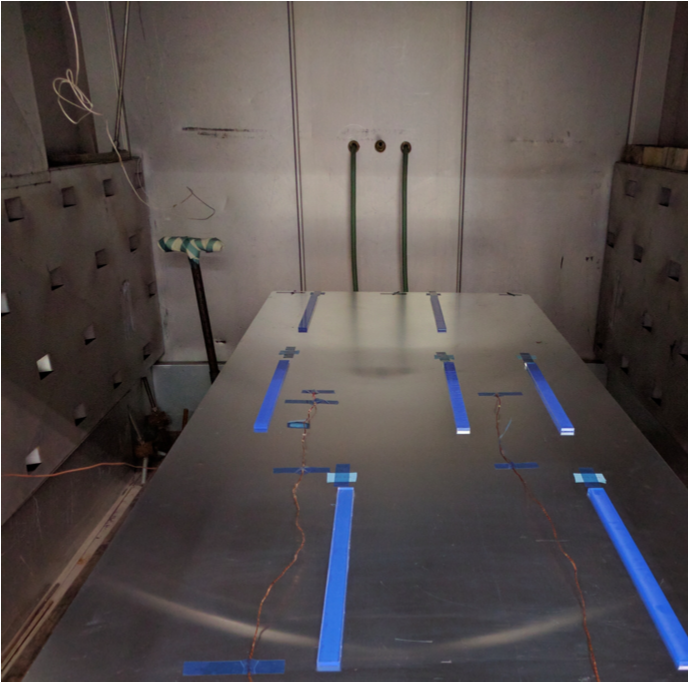
\includegraphics[height=7cm]{pds-dipannealpic.png}
 % 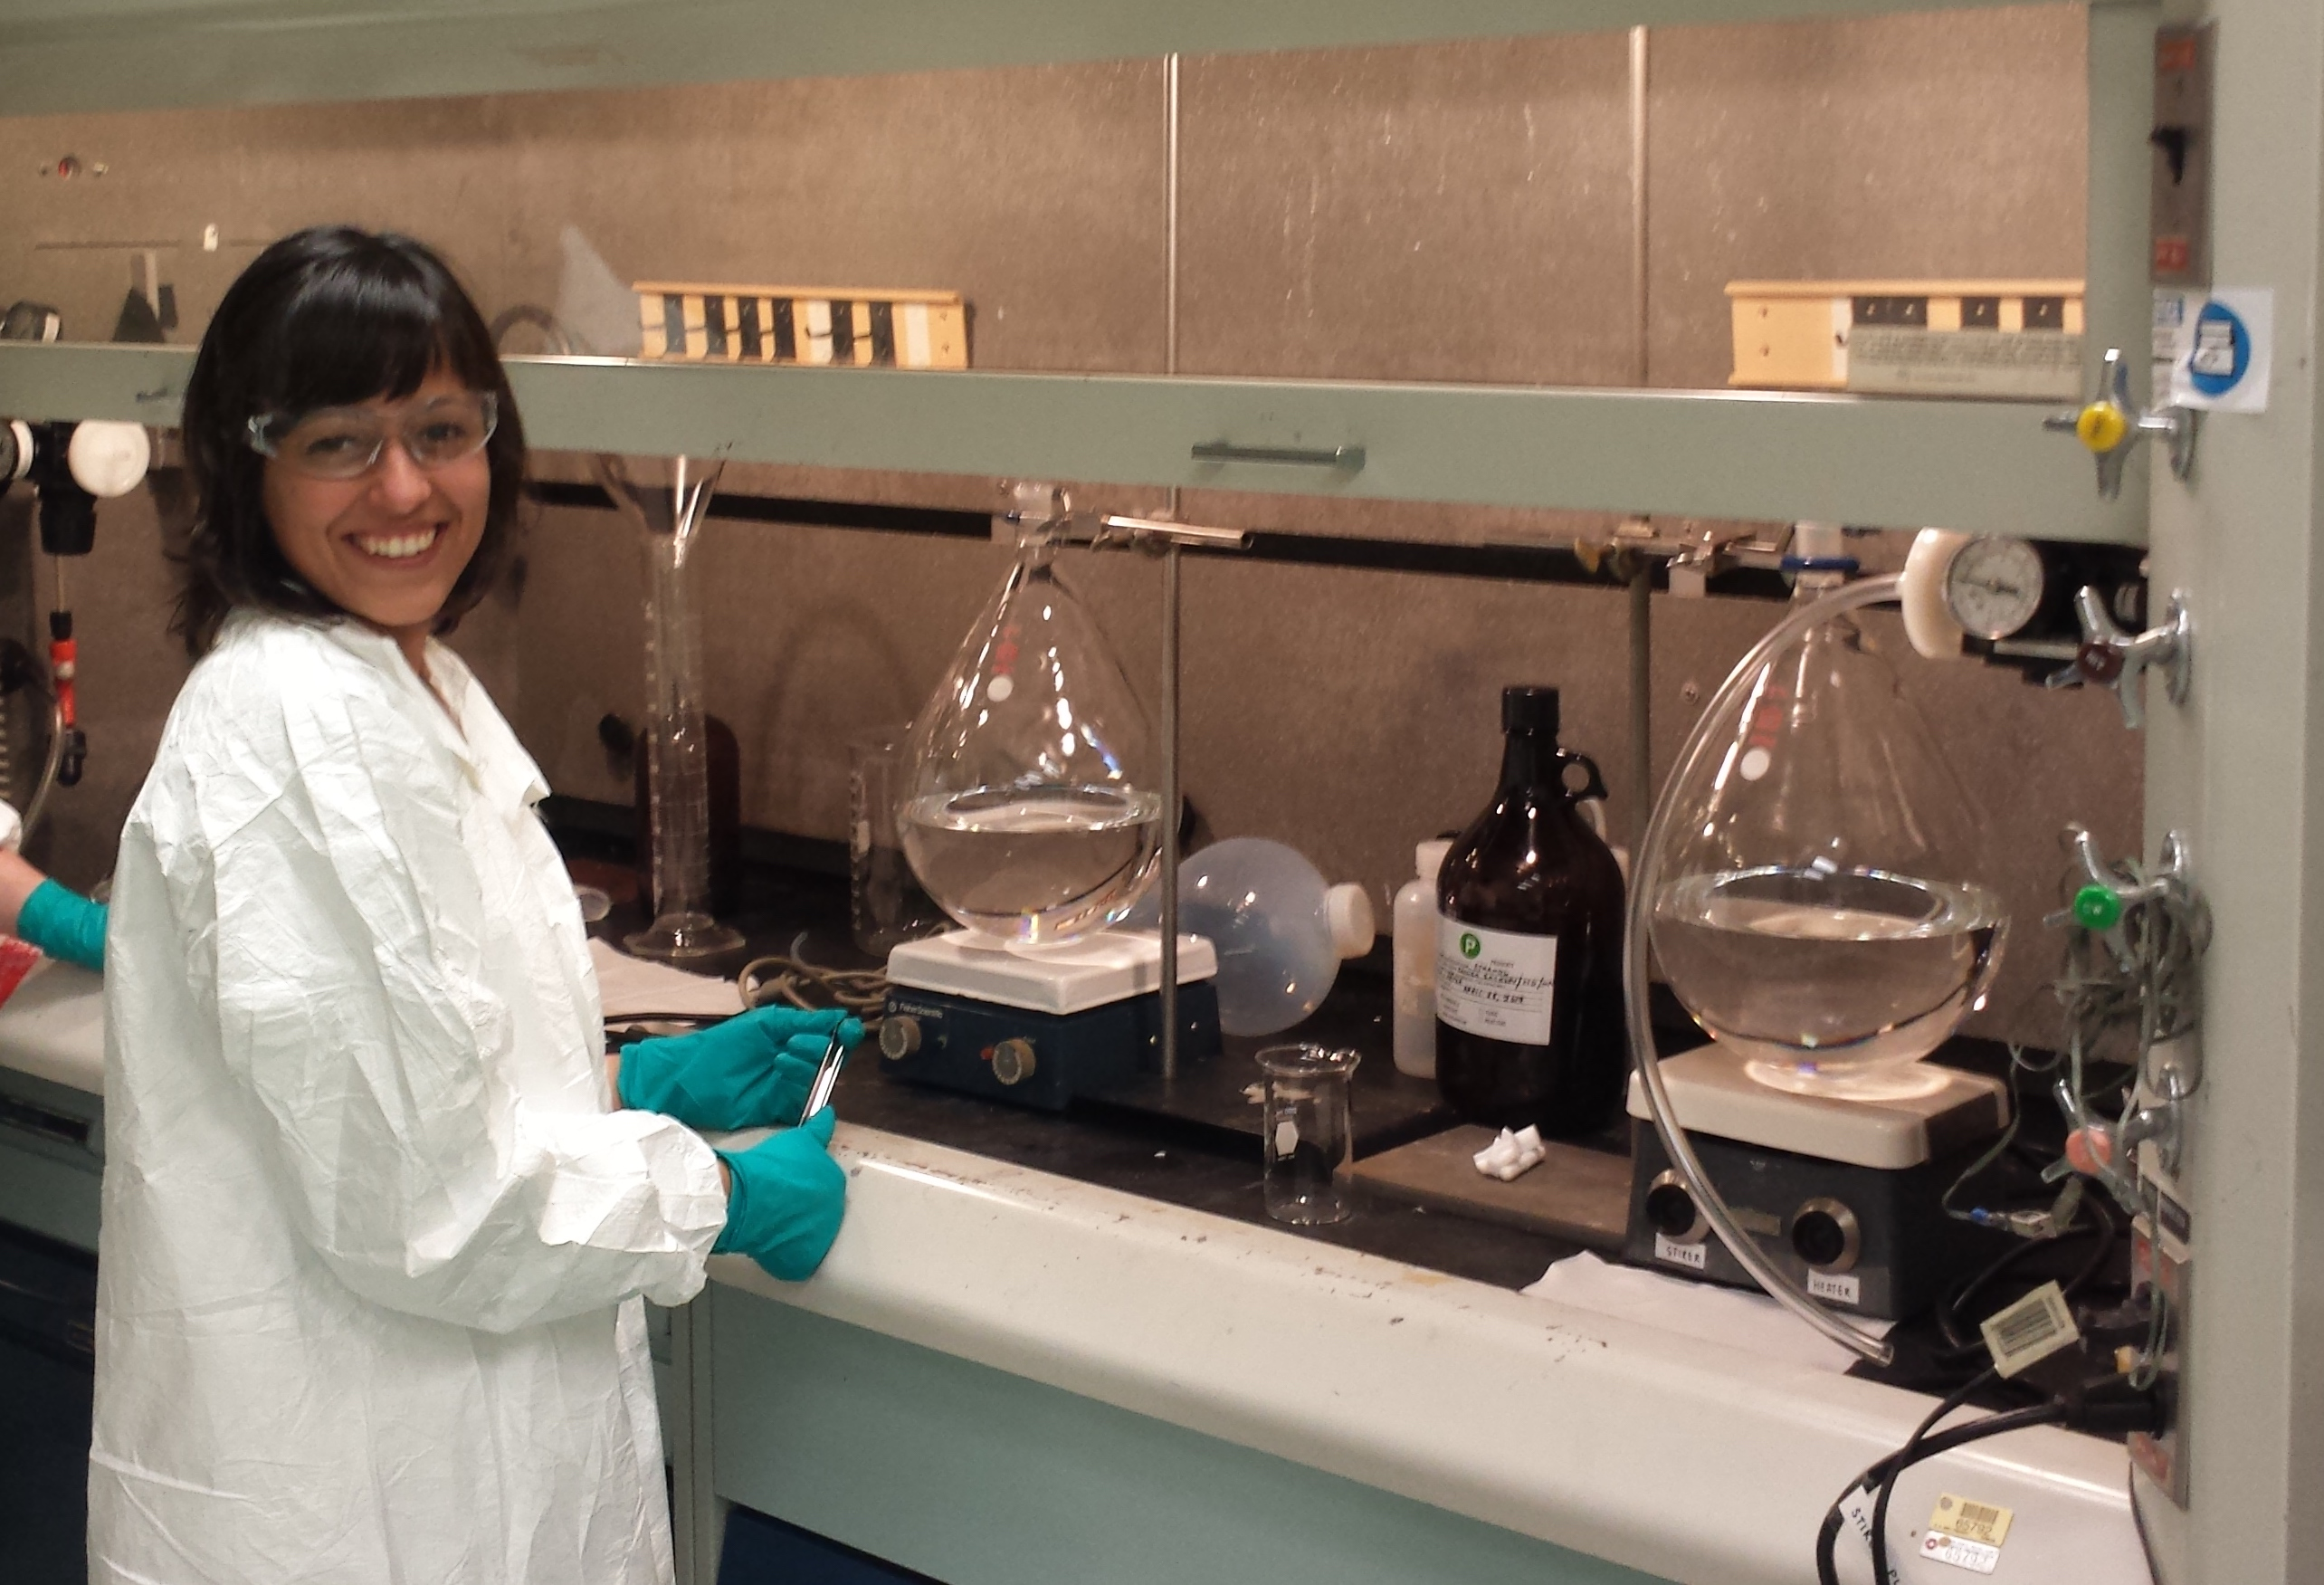
\includegraphics[width=0.4\columnwidth]{pds-dipmixpic.jpg}.  \\
 % 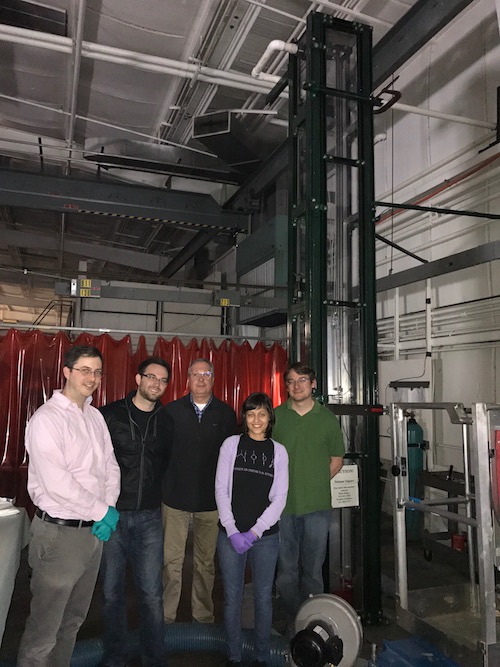
\includegraphics[width=0.4\columnwidth]{pds-dipvesselpic.jpg}
  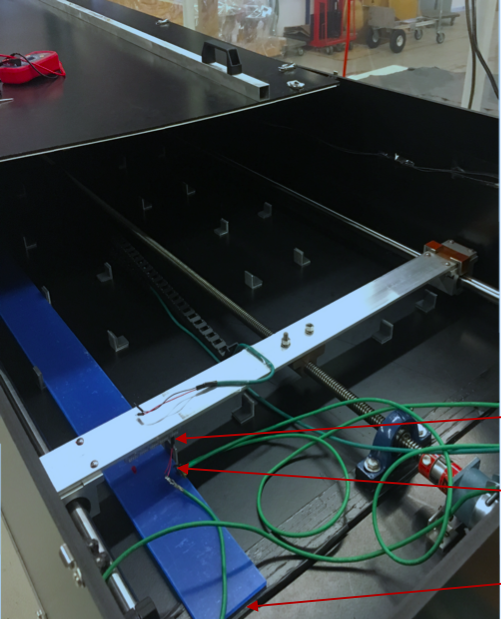
\includegraphics[height=7cm]{pds-dipdarkboxpic.png}
\end{dunefigure}


%%%%%%%%%%%%%%%%%%%%%%%%%%%%%%%%%%%


\subsubsection{Double-Shift Light Guides}
\label{ssec:fdsp-pd-pc-prod-bar2}

The production and assembly of the double-shift light guide modules has two main components; the wavelength-shifting plates and the EJ-280 light guides. Many of the production, quality assurance, and assembly procedures developed for the double-shift light guide design deployed at ProtoDUNE-SP will remain the same for the DUNE single-phase far detector.
													
%\paragraph*{Manufacture of the WLS Plates}
\paragraph*{WLS Plates}

%^%^%^%^%
Sheets of 1/16''-thick UVT acrylic purchased from McMaster-Carr\footnote{https://www.mcmaster.com} are laser-cut into \SI{77}{cm}$\times$\SI{9}{cm} templates with two \SI{34.2}{cm}$\times$\SI{8.6}{cm} plates per template (Figure~\ref{fig:pds-doubledhiftlg-plate}~(top)). Each template also includes three small \SI{3.81}{cm}$\times$\SI{2.54}{cm} pop-out tabs on either side of and between the two plates. After the acrylic templates are coated with TPB these tabs are separated from the plate and tested in a VUV monochromator to determine the quality of the coating on the two associated plates.

\begin{dunefigure}[Dip-coated acrylic plates.]
{fig:pds-doubledhiftlg-plate}
{A laser-cut acrylic template holding two plates and three test tabs (top). TPB-coated acrylic plates after spraying during fabrication of parts for ProtoDUNE-SP (bottom).}
    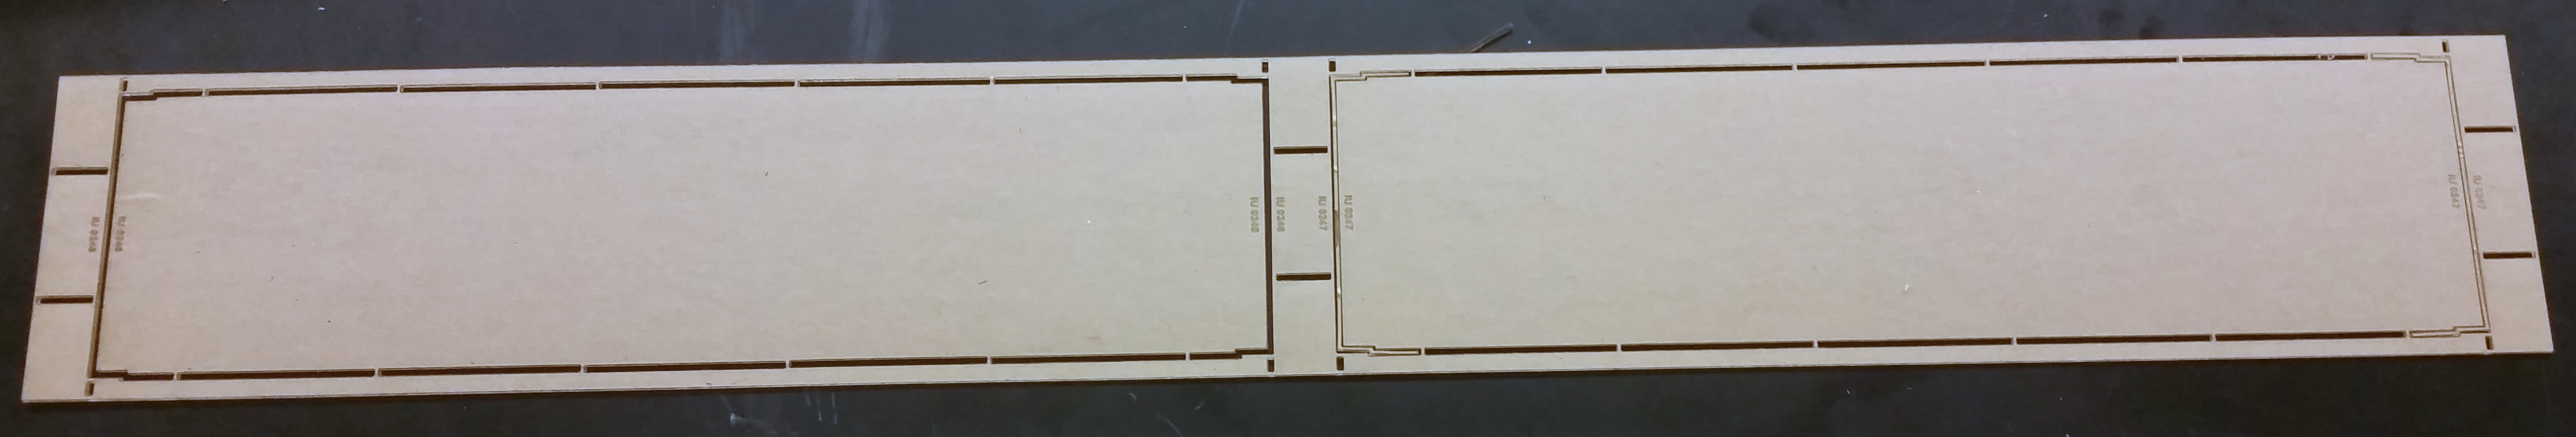
\includegraphics[width=0.7\columnwidth]{pds-doubledhiftlg-acrylictemplate.jpg}\\
    \vspace{0.3cm}
    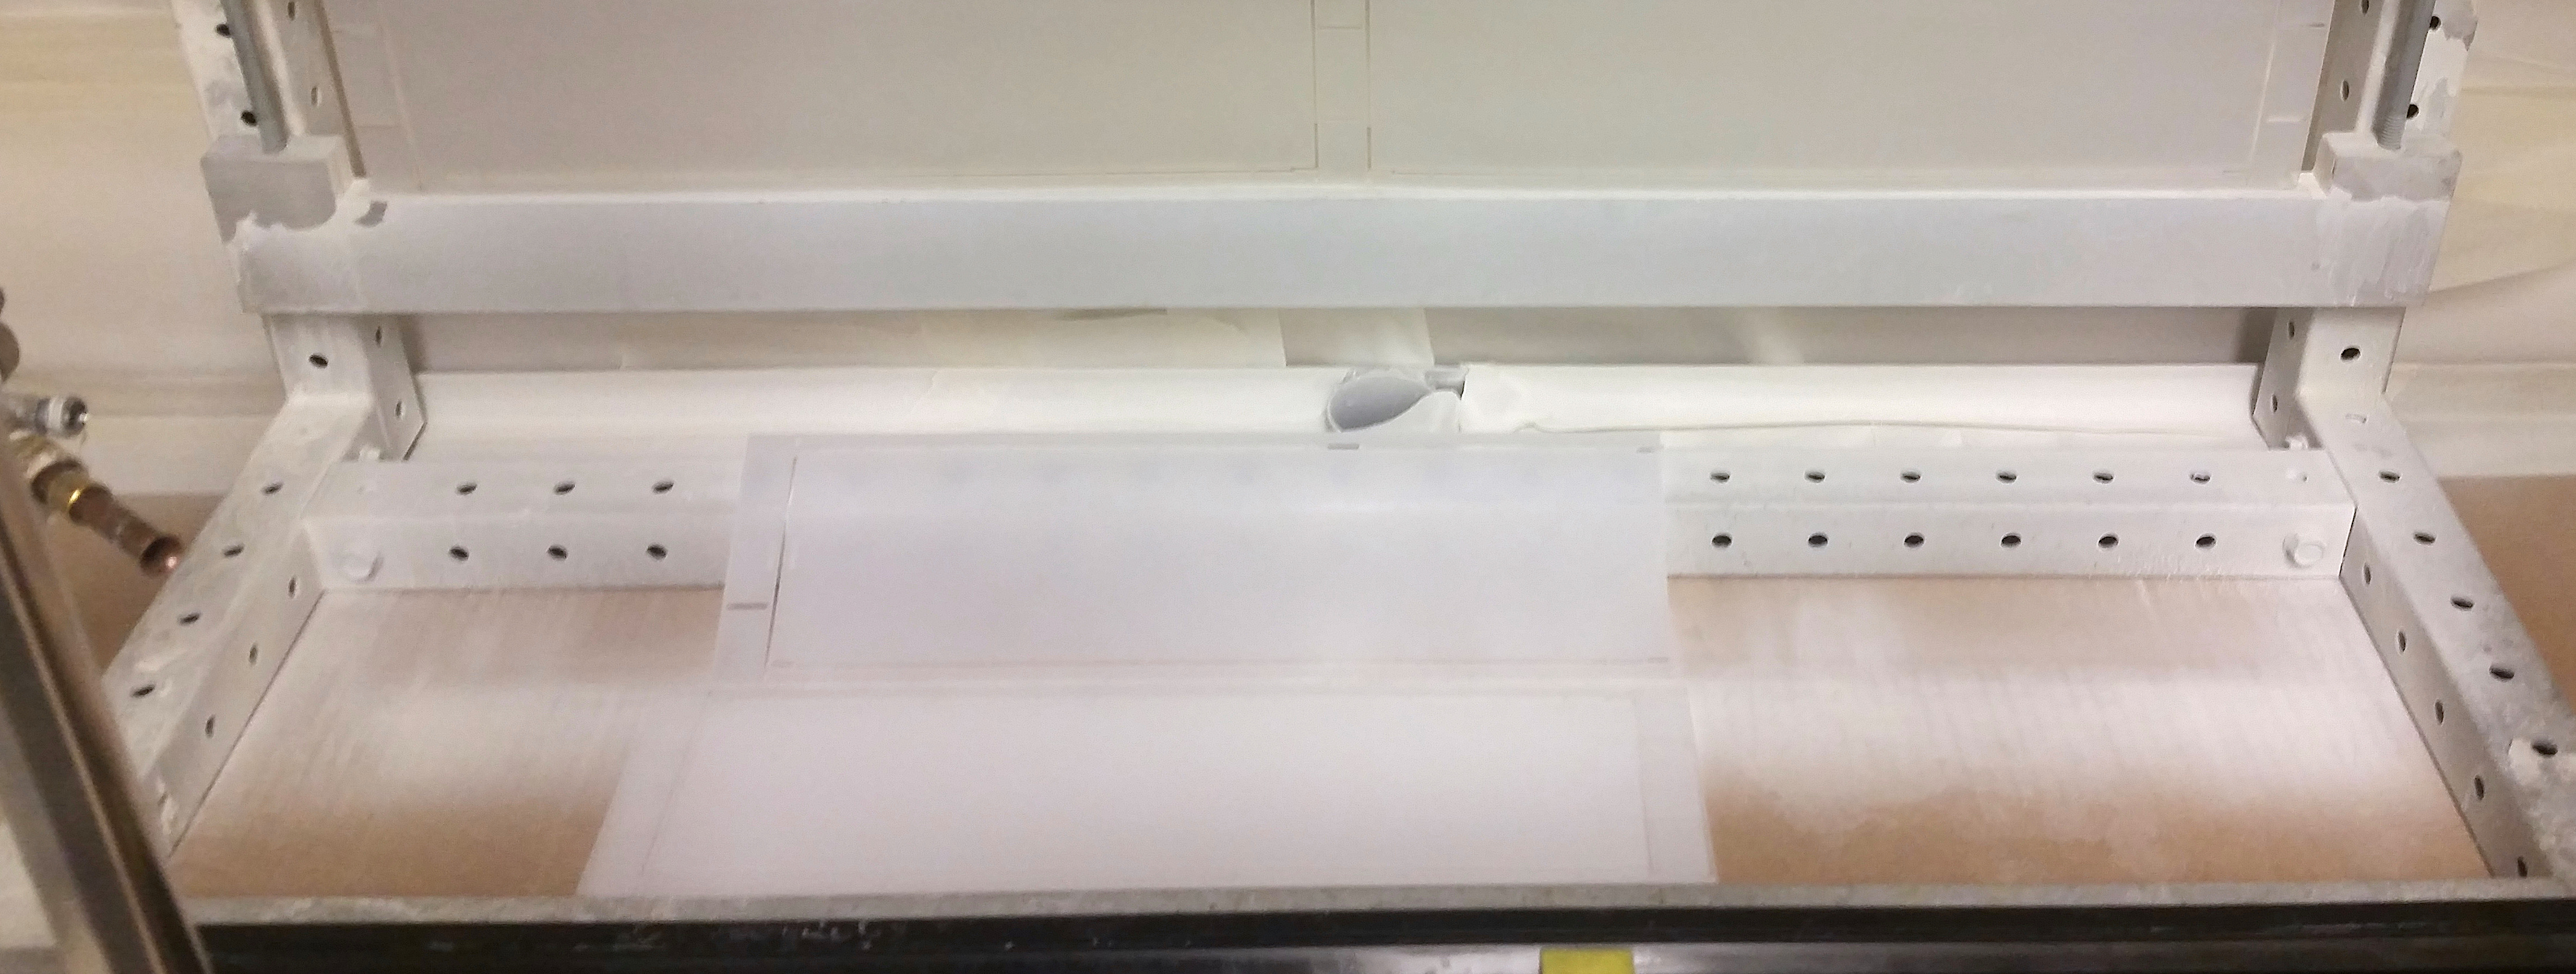
\includegraphics[width=0.7\columnwidth]{pds-doubledhiftlg-sprayedplates.jpg}
\end{dunefigure}

Scintillation grade ($\ge 99$\%) TPB is dissolved in dichloromethane (DCM) at a ratio of \SI{5}{g} TPB per \SI{1000}{g} DCM. The solution is applied to the templates using a high-volume low-pressure (HVLP) sprayer system under a fume hood. The relatively small number of plates manufactured for ProtoDUNE-SP were sprayed by a technician to approximate an established standard coating thickness measured to have an acceptably high VUV photon conversion efficiency. Figure~\ref{fig:pds-doubledhiftlg-plate}(bottom) shows the HVLP spray-coating mount with a coated acrylic template. Two plates and three test tabs can be seen in the HVLP mounting frame. A second sprayed template has been broken at one of the midpoint cuts and positioned in the photo. For SPFD production, the spray-coating process will be automated or commercialized to accommodate the large-scale production necessary for the DUNE single-phase far detector.

After spraying, the acrylic templates are baked in a vacuum oven at 80$^{\circ}$C overnight, just below the glass transition point of acrylic. The softened acrylic partially absorbs the TPB into the surface, better affixing the wavelength-shifting coating. Uneven heating during the baking process described above can deform the coated plates, but this is minimized by careful oven fixturing to ensure even heating. After baking, the dimensions of the samples are measured and only plates within the production tolerance are accepted for further testing.
%\paragraph*{QA of the WLS Plates}
To ensure adequate and uniform performance of the coated plates, the conversion efficiency is tested using a VUV monochromator. During ProtoDUNE-SP production, plates were fabricated and tested 
%at Indiana University 
using a McPherson\footnote{http://mcphersoninc.com} VUV monochromator with deuterium lamp source to study performance at 128~nm. The full plates were too large for the sample chamber
% of the Indiana University 
VUV monochromator system, so the testing tabs on either side of each plate were used to constrain the plate's performance. 
%VUV monochromator system, so the two testing tabs on either side of each plate were used to constrain the plate's performance. 
%VUV photons at 128~nm are selected by the monochromator and directed toward the test tabs. The photocurrent from a SiPM behind the sample is measured. Before and after sample testing, the intensity of the lamp output at 128~nm is measured with a VUV-sensitive photodiode and no sample. The ratio of the dark-subtracted SiPM photocurrent to the dark-subtracted VUV photodiode photocurrent is proportional to the absolute conversion efficiency of the sample. The average of this ratio between the two neighboring test tabs is taken as an estimate of the conversion performance of a plate.
Only plates that exhibit a relative efficiency above an acceptance threshold are shipped to the assembly facility for deployment along a light guide. For ProtoDUNE-SP, a threshold was chosen to accept plates that were comparable or superior to those studied at the Blanche test stand~\cite{bib:DoubleShiftLG-NIM-171113} described previously.

%\paragraph*{Receipt and QA of the Light Guides}
\paragraph*{WLS-Doped Light Guides}

The EJ-280 light guides are fabricated and cut to length by Eljen Technologies. Upon receipt, each light guide is unpacked, visually inspected for defects, checked for dimensional tolerance, and scanned using a \SI{430}{nm} LED to determine its attenuation length in air (Figure~\ref{fig:pds-doubleshiftlg-ej280}). 
Since the index of refraction for $\sim$\SI{500}{nm} light in LAr is larger than in air and the critical angle for trapping by total internal reflection is correspondingly lower, so attenuation scans of sample light guides were made in both air and liquid argon (using a movable Am-241 $\alpha$ source) to quantify the correlation between measurements in air and in LAr.  Attenuation lengths longer than $\sim$5~meters measured in the darkbox correspond to attenuation lengths in LAr longer than $\sim$2~meters. An acceptance threshold of 5~meters measured at both ends of an EJ-280 light guide in the darkbox ensures adequate attenuation performance for the modules deployed in the DUNE detectors.

%Each light guide is placed on a temperature-controlled metrology table where width, length, and thickness measurements are taken. Light guides within tolerance in these dimensions are then scanned in a long darkbox using a 430~nm LED~(Fig.~\ref{fig:pds-doubleshiftlg-ej280}). Optical photodetectors are placed at each end of the light guide and a third is located on the opposite side of the light guide to the LED. The LED is moved to different positions along the light guide using a stepper motor. The attenuation characteristics of the light guide are determined by comparing the relative signal measured at the end of the light guide as the LED is moved to different positions. Two attenuation curves are measured for each light guide, corresponding to readout at each end. The third photodetector travels with the LED to confirm the uniformity of the wavelength shifting response across the light guide.
%Attenuation scans of EJ-280 light guides in the darkbox and in liquid argon (using a movable Am-241 $\alpha$ source) performed at Indiana University have demonstrated the correlation between attenuation lengths measured in air and in LAr. The index of refraction for $\sim$500~nm light in LAr is larger than in air and the critical angle for trapping by total internal reflection is correspondingly lower. Attenuation lengths longer than $\sim$5~meters measured in the darkbox correspond to attenuation lengths in LAr longer than $\sim$2~meters. An acceptance threshold of 5~meters measured at both ends of an EJ-280 light guide in the darkbox ensures adequate attenuation performance for the modules deployed in the DUNE detectors.

\begin{dunefigure}[EJ-280 light guide in darkbox for attenuation scan QA.]{fig:pds-doubleshiftlg-ej280}
{EJ-280 light guide in a dark box for attenuation scan QA at Indiana University (prepared for ProtoDUNE-SP).}
  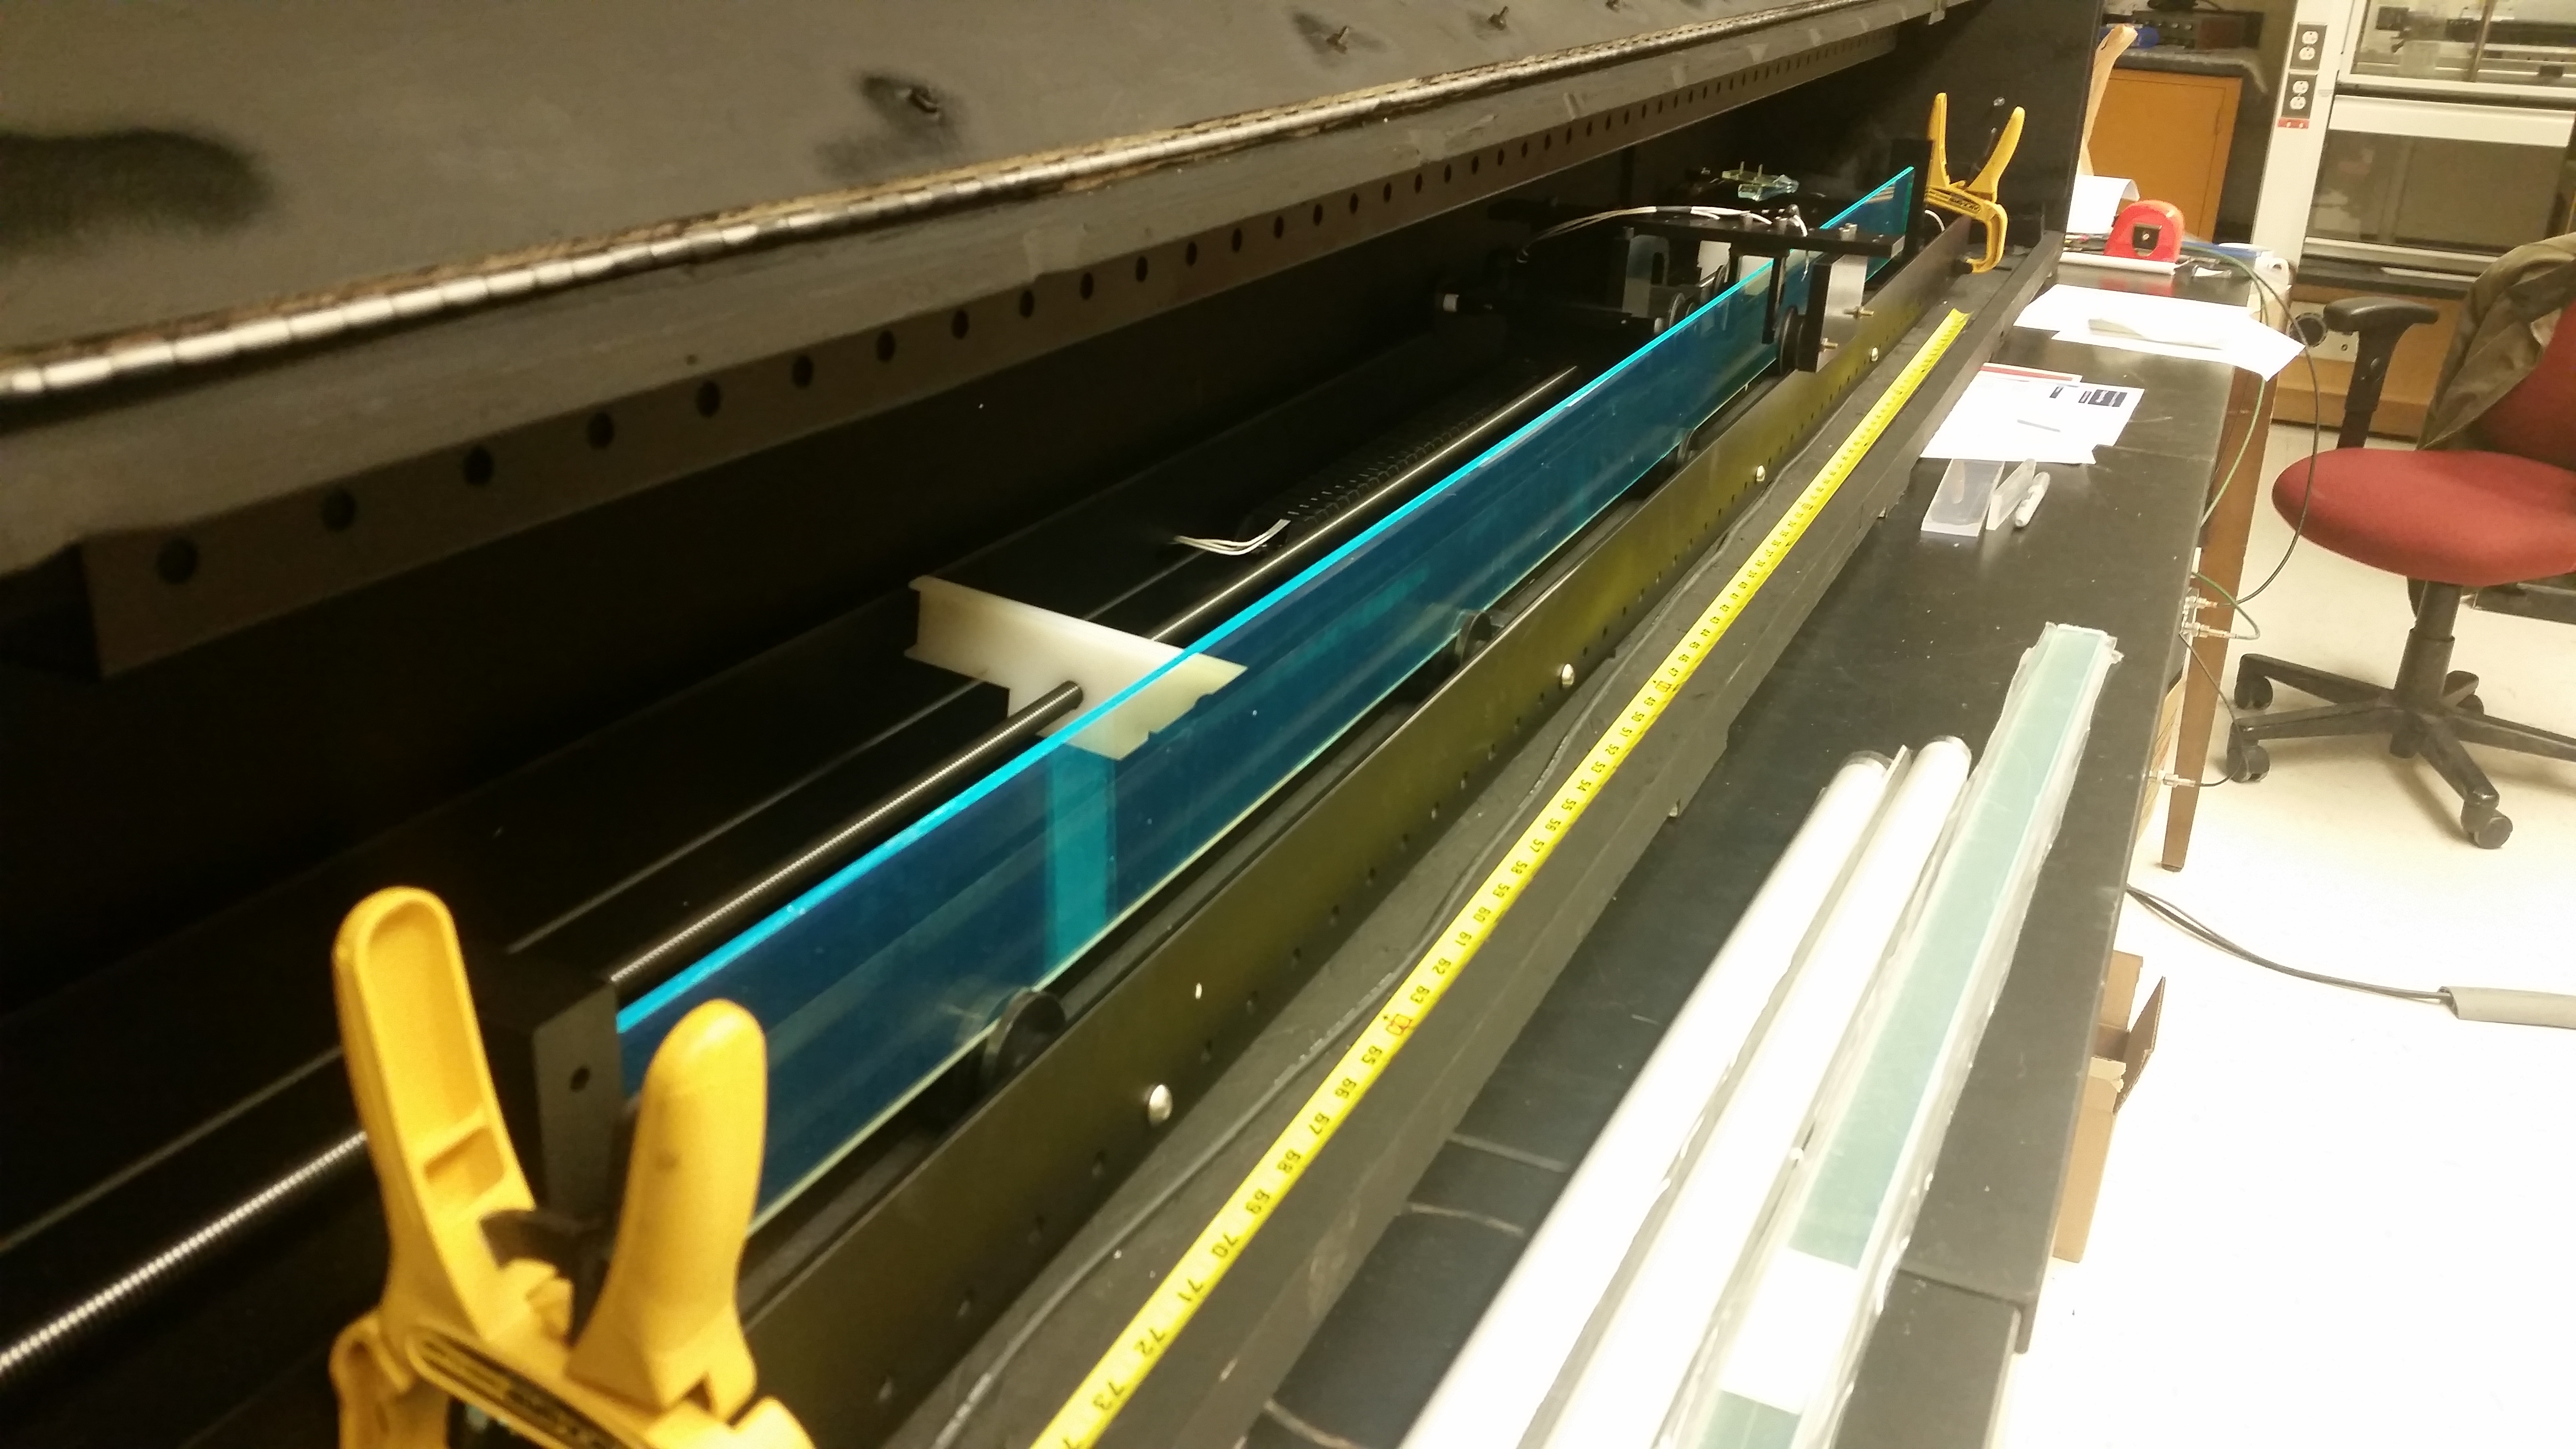
\includegraphics[width=0.6\columnwidth]{pds-doubleshiftlg-ej280.jpg}
\end{dunefigure}

Visual inspection of light guides received for ProtoDUNE-SP found multiple instances of fogging or mottling on the surface and within the bulk of some light guides. However, these features did not appear to impact the attenuation properties or uniformity during darkbox scans. Acceptance of light guides for shipment to the assembly facility was based on the metrology and attenuation results.

%\paragraph*{Assembly of the Double-Shift Light Guide Module}

%Parts are shipped to the assembly point where the EJ-280 light guide is mounted into the module frame and the WLS plates are attached as illustrated in Figure~\ref{fig:pds-doubleshiftlg-platemounting}

%\begin{dunefigure}[Mounting of the WLS plates to the EJ-280 bar.]{fig:pds-doubleshiftlg-platemounting}
%{Mounting of the WLS plates to the EJ-280 bar.}
%  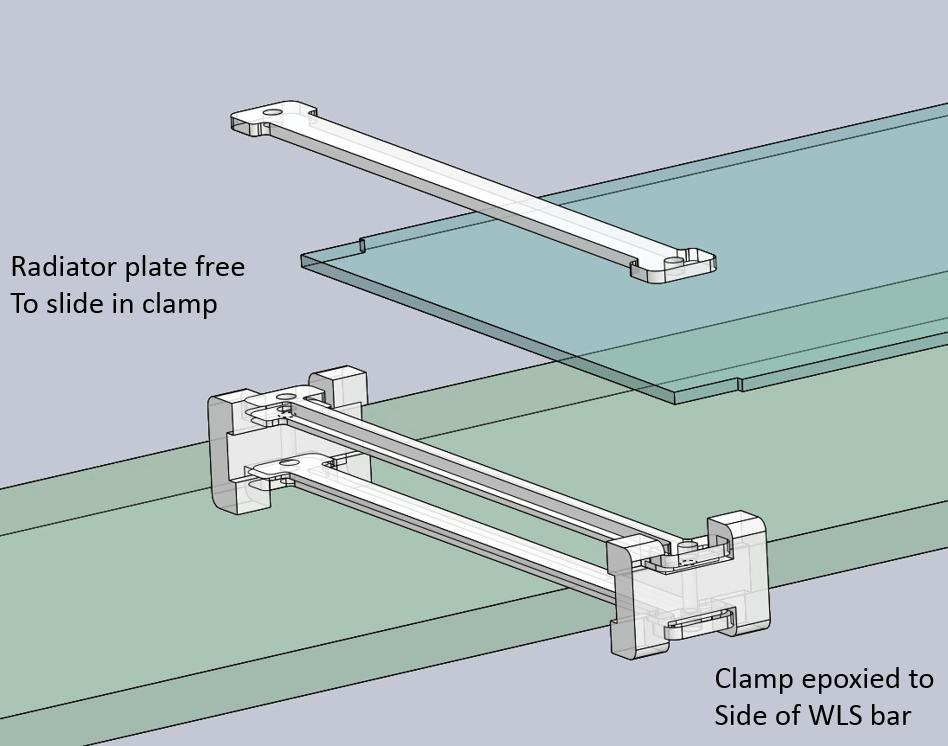
\includegraphics[width=0.3\columnwidth]{pds-doubleshiftlg-platemounting.jpg}
%\end{dunefigure}


% DW 2/23/18
%^%^%^%^%

%%%%%%%%%%%%%%%%%%%%%%%%%%%%%%%%%%%%%
% Dave 2/21/18 - Common assembly
\subsection{Photon Detector Module Assembly}

Final assembly planning for photon detector modules is guided by the assembly of \num{60} ProtoDUNE-SP PD modules (representing multiple units of all three varieties) at the Colorado State University assembly facility.  SPFD assembly will occur at one or more assembly facilities, (number and location to be determined prior to the TDR).  Several features of this are common to all three types of module, and these aspects will be covered in this section.

\subsection{Incoming Materials Control}

All materials for PD module assembly will be delivered with a previously generated QC traveller (in the case of materials custom fabricated for DUNE) or will have an incoming materials traveller generated immediately upon receipt of the component (for commercial components).  These travelers will be scanned upon receipt at the assembly facility, and the data stored in the DUNE QC database.  Materials will either arrive with a pre-existing DUNE inventory control batch/lot number, or will have one assigned prior to entering the assembly area.  Bar code labels attached to storage containers for all components in the assembly area will facilitate traceability throughout the assembly process.

Immediately upon receipt all materials will undergo an incoming materials inspection, including confirmation of key dimensional tolerances as specified on the incoming materials documentation for that component.  The results of these inspections will be included on the traveller for that batch/lot and entered into the database.

In the case of discrepancy, the deviation from nominal will be recorded in an exception section of the traveller, as well as the resolution of the discrepancy.

\subsection{Assembly Area Requirements}

Assembly will occur in a class \num{100000} or better clean assembly area.  Photosensitive components (TPB coated surfaces) are sensitive to near-UV light exposure, and will be protected by blue-filtered light in the assembly area (>\SI{400}{nm} or better filters\footnote{For example, GAMTUBE T1510 from GAM Products, Inc. - http://www.gamonline.com/catalog/gamtube/index.php}); it has been determined that this level of filtering is sufficient to protect coated surfaces during  exposures of up to several days. For exposures of weeks or months, such as in the ProtoDUNE cryostat assembly area, a higher cut-off yellow filter is used\footnote{F007-010 Amber with Adhesive - http://www.epakelectronics.com/uv\_filter\_materials\_flexible.htm.}. 
The requirement for light exposure is to be revisited prior to SPFD production.

% 4/12/18 per Dave reporting on Stu's studies?

Exposure of photosensitive components will be strictly controlled.  Work flow will be restricted to ensure no component exceeds a total exposure of \SI{8}{hours} to filtered assembly area lighting (including testing time).

\subsection{Component Cleaning}

All components will be cleaned  as appropriate, following manufacturer's specifications and DUNE materials test stand recommendations.  Cleaning procedures will be written for all incoming materials, and completion of these procedures noted in the appropriate travelers.

\subsection{Assembly Procedures}

Following the example of the ProtoDUNE-SP experience, detailed, step-by-step written procedure documents will be followed for each module, and a QC traveller for each module is completed and recorded in the database.  ProtoDUNE-SP experience suggests that a two-person assembly team is necessary and sufficient for all three currently-considered versions of the light collector modules.  Our current assembly plan envisions two 2-person teams operating at the same time, with a fifth person acting as shift leader.  The shift leader is not directly involved in assembly, but rather acts as a QC officer responsible primarily for ensuring distributing materials to the assembly teams (documenting the batch/lot numbers for each detector on the relevant module travelers) and ensuring that documented assembly procedures are followed.

Assembly fixtures mounted to \SI{2.4}{m} long flat optical tables will be used to support and align PD components during assembly.  All workers handling PD components will wear gloves, hair nets, shoe covers, and clean room disposable lab jackets at all times.

%\fixme{(Insert 3 pictures here, of all 3 module types being assembled at CSU)}

%\begin{dunefigure}[Photo of Dip-Coated Bar Prototype Assembly.]{fig:photoDip}
%{Photo of Dip-Coated Bar Prototype Assembly.}
%  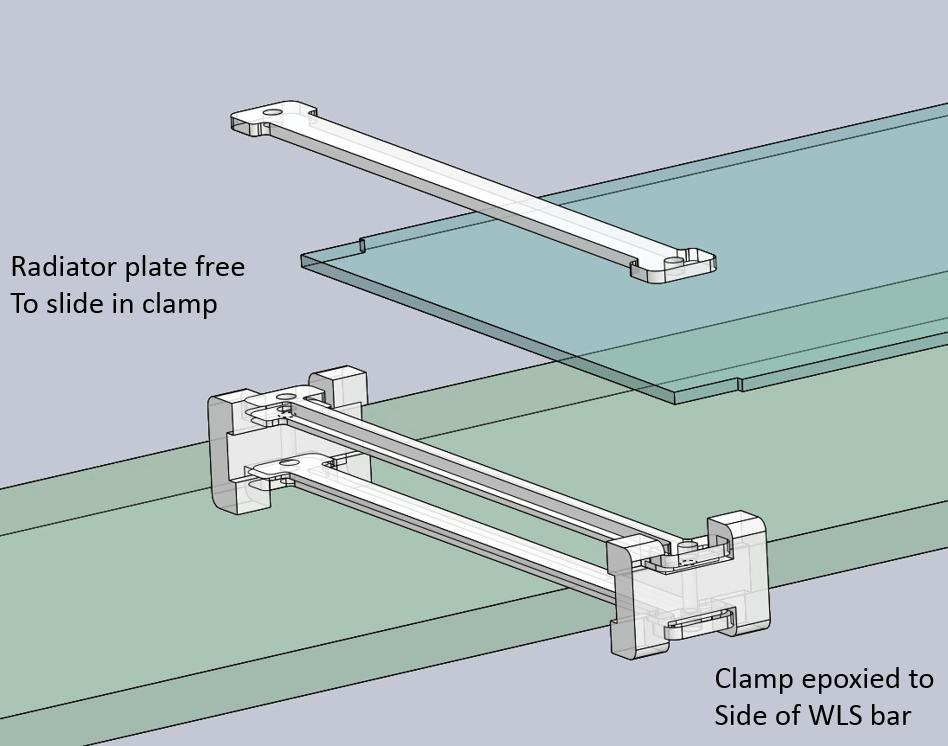
\includegraphics[width=0.5\columnwidth]{pds-DoubleShiftLG-PlateMounting.jpg}
%\end{dunefigure}

%\begin{dunefigure}[Photo of Double-Shift Bar Prototype Assembly.]{fig:photoDouble}
%{Photo of Double-Shift Bar Prototype Assembly.}
%  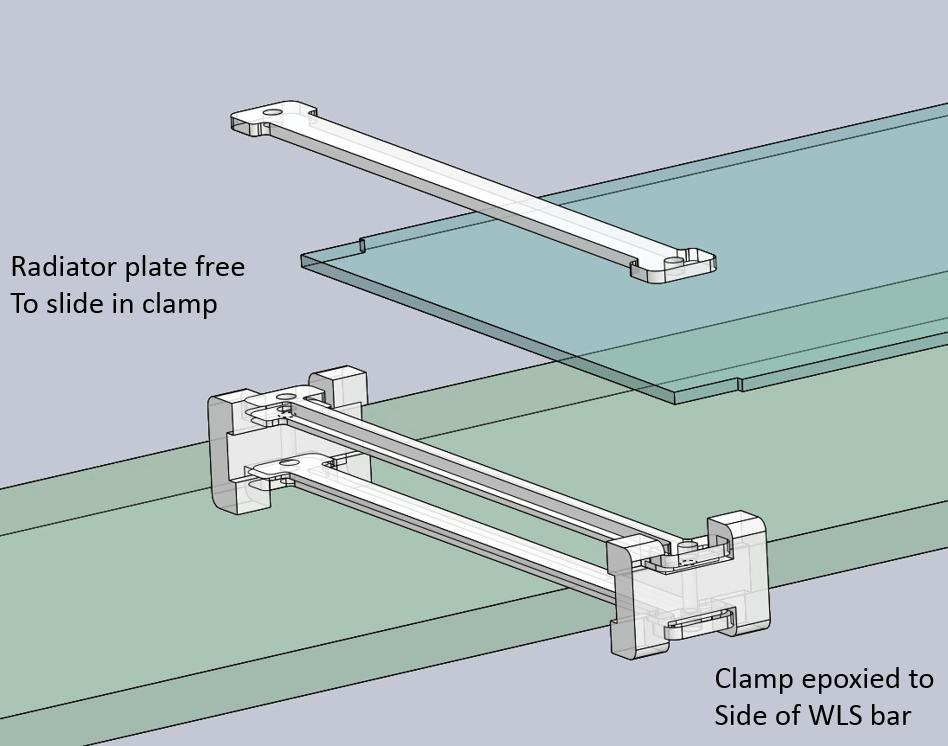
\includegraphics[width=0.5\columnwidth]{pds-DoubleShiftLG-PlateMounting.jpg}
%end{dunefigure}

%\begin{dunefigure}[Photo of ARAPUCA Bar Prototype Assembly.]{fig:photoARAPUCA}
%{Photo of ARAPUCA Bar Prototype Assembly.}
%  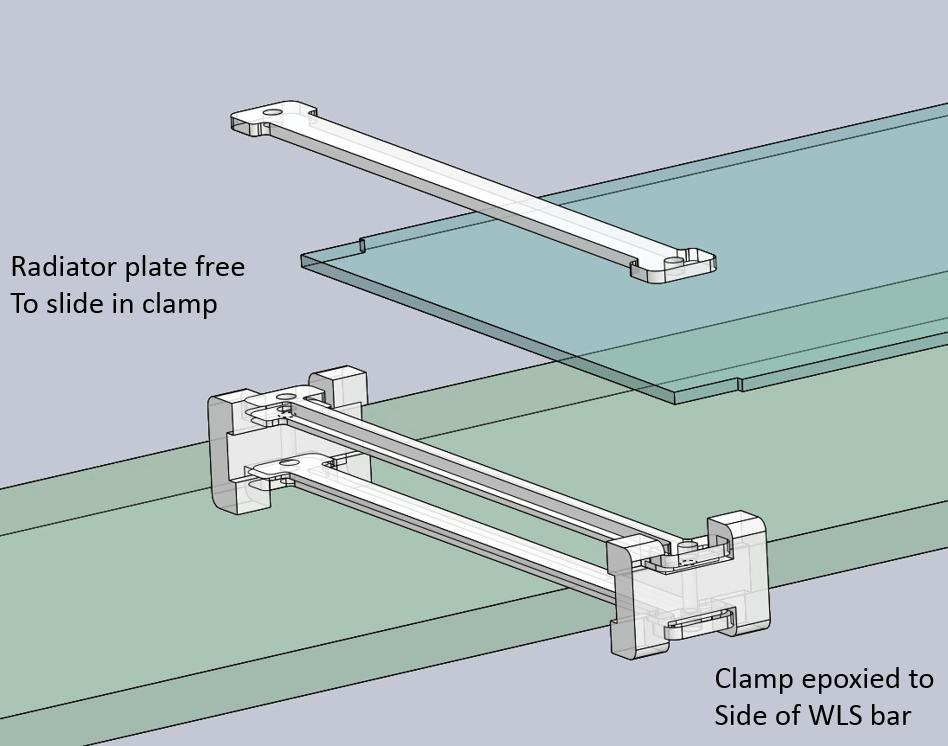
\includegraphics[width=0.5\columnwidth]{pds-DoubleShiftLG-PlateMounting.jpg}
%\end{dunefigure}


\subsection{Post-Assembly Quality Control}

Post-assembly QC planning is currently based on ProtoDUNE-SP experience, modified as appropriate for larger-scale production.  Each module will go through a series of go-no gauges designed to control tolerances of critical interface points.  Following this, each module will be inserted into a test APA support model, representing the tightest slot allowed by APA mechanical tolerances. Next, each module will be scanned at a fixed set of positions (to be determined prior to the TDR) with \SI{275}{nm} UV LEDs.  The detector response at each position will be read out using PD readout electronics, and the data compared to pre-established criteria.  Figure~\ref{fig:pds-pd-scanner} is a photograph of the scanner used for ProtoDUNE-SP modules. These performance data will serve as a baseline for the module, and will be compared against those taken in an identical scanner shortly before installation into the APA, as in the ProtoDUNE-SP experience.  All data collected will be recorded to the module traveler and to the DUNE QC database.
As a final QC check, post-assembly immersion into a LN2 cryostat followed by a repeat scan of each PD module (as in ProtoDUNE-SP) is being considered.

\begin{dunefigure}[PD module scanner.]{fig:pds-pd-scanner}
{PD module scanner.}
  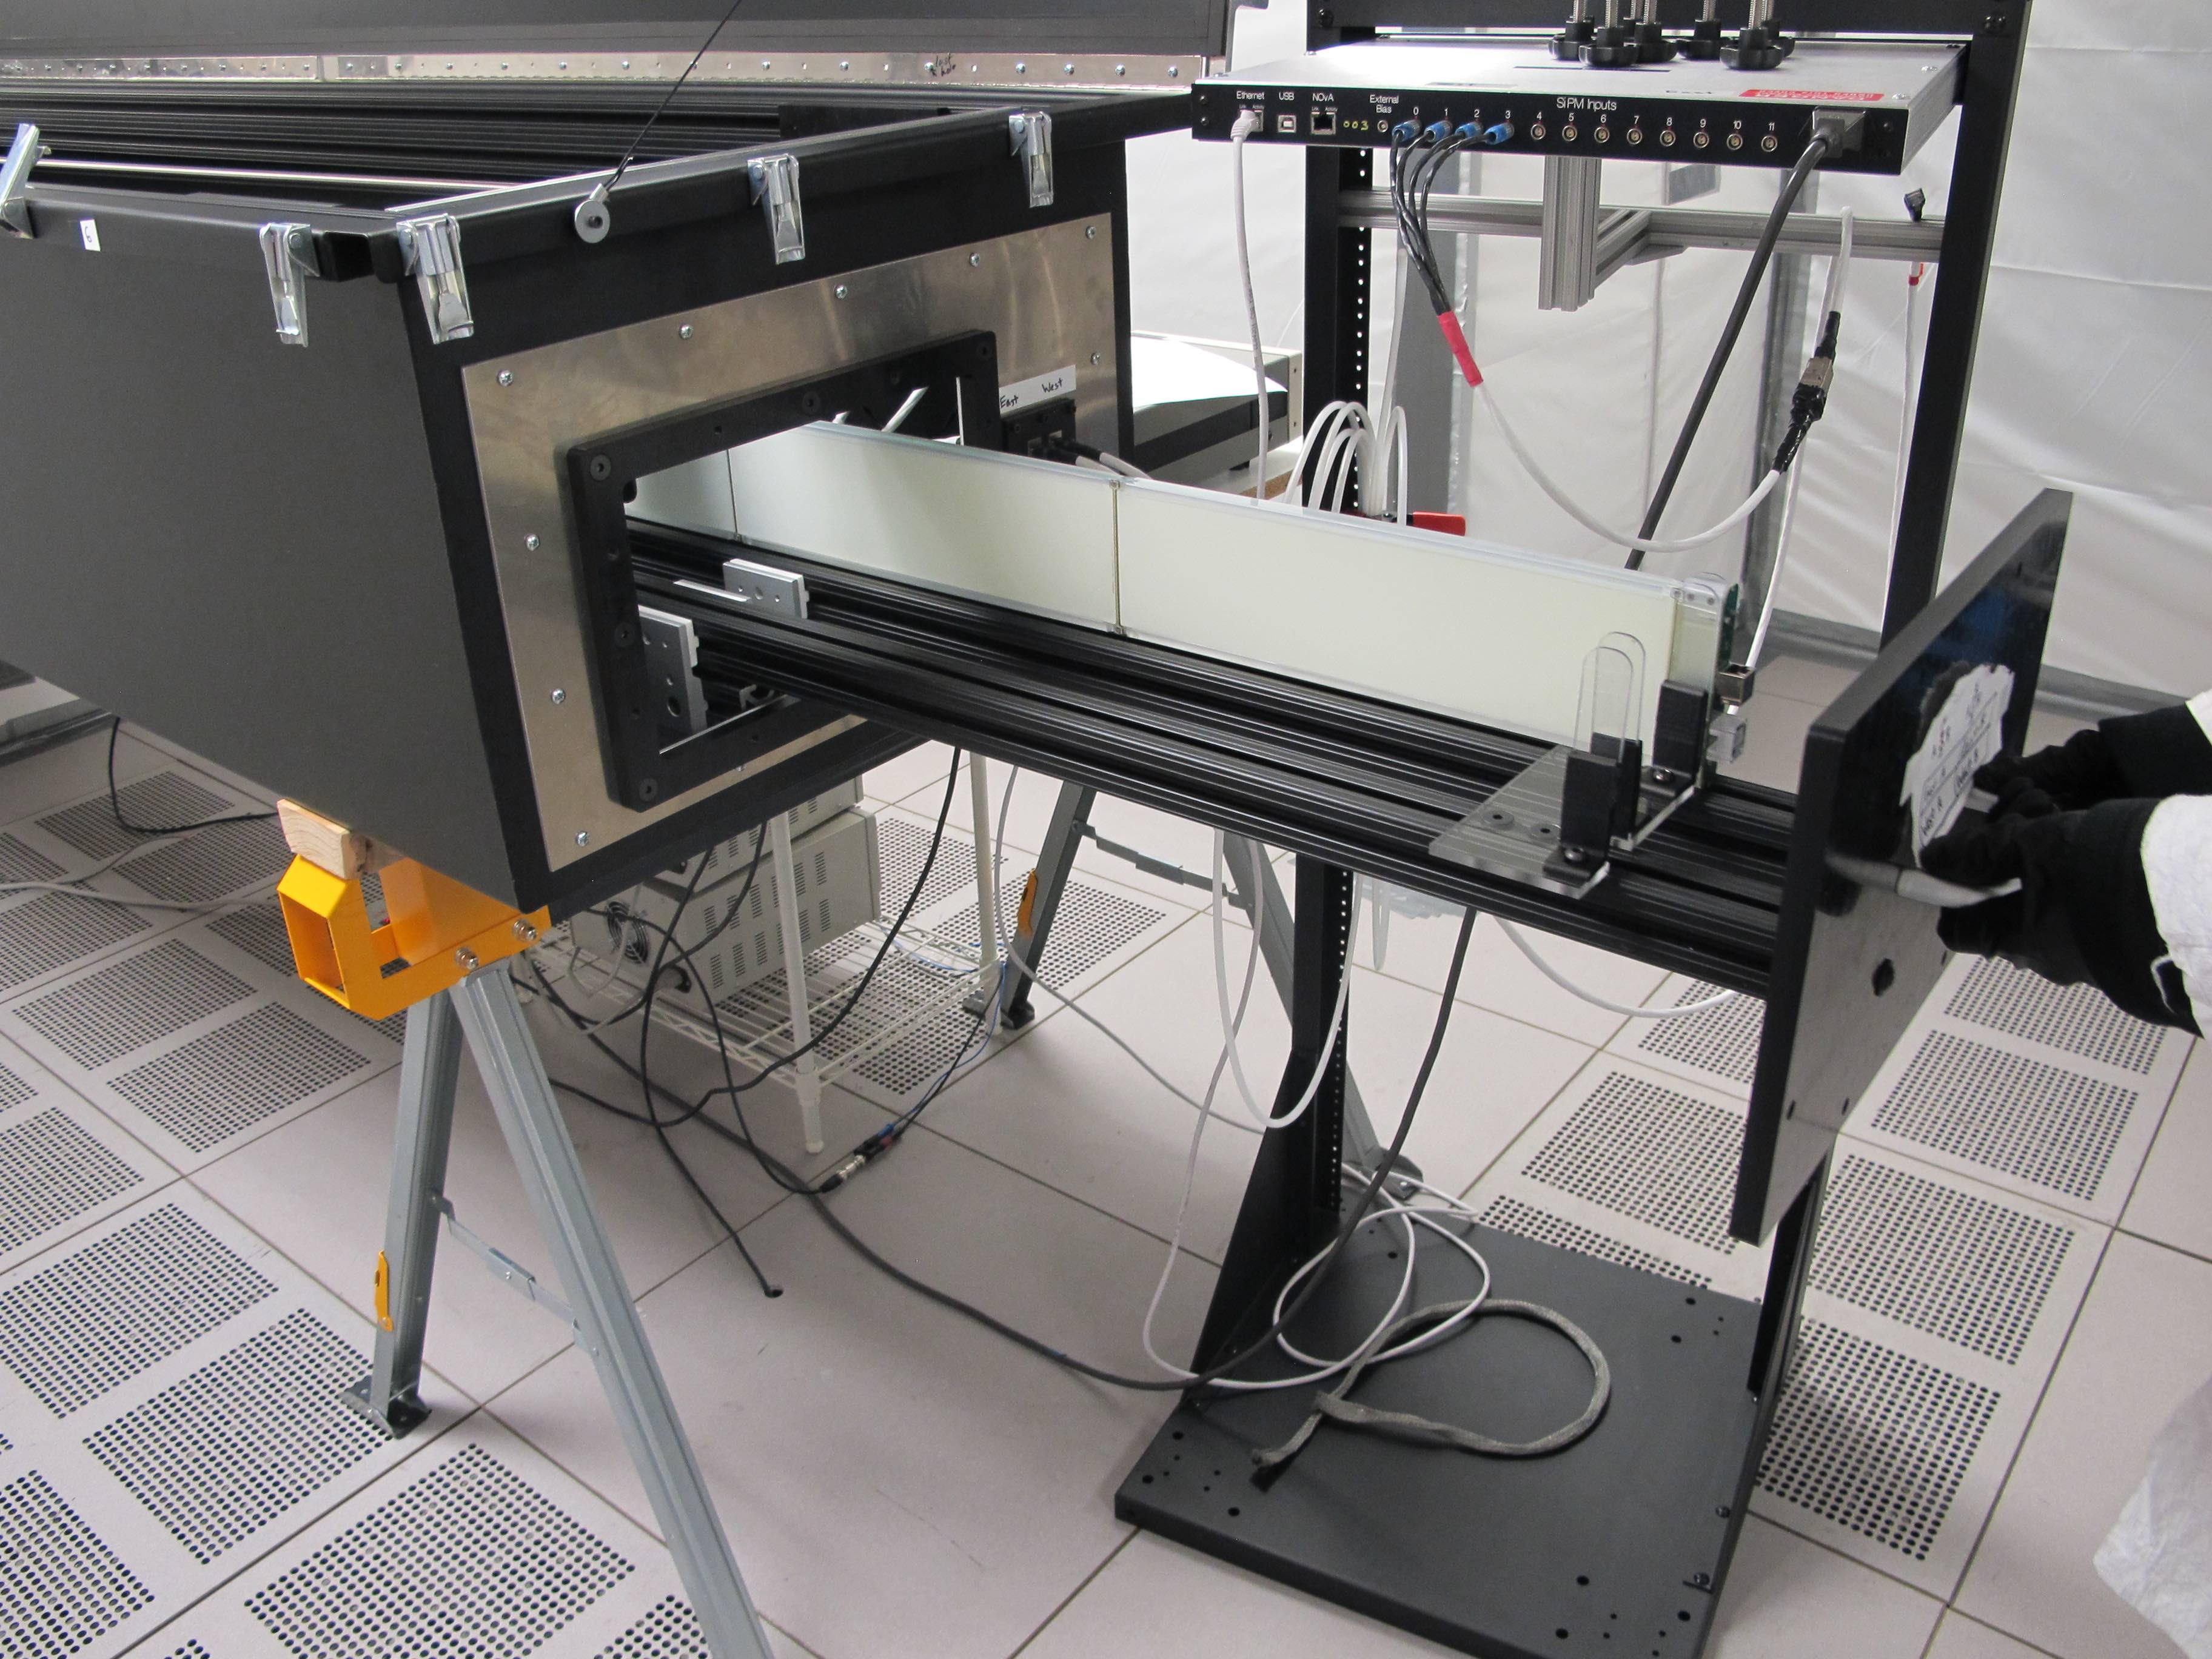
\includegraphics[width=0.6\columnwidth]{pds-pd-scanner.jpg}
\end{dunefigure}


% End Dave 2/21/18
%%%%%%%%%%%%%%%%%%%%%%%%%%%%%%%%%%%%%


%%%%%%%%%%%%%%%%%%%%%%%%%%%%%%%%%%
\subsection{APA Frame Mounting Structure and Module Securing}	
\label{sec:fdsp-pd-assy-frames}
%\todo{\color{blue} Content:  Warner}

Photon detector (PD) modules are inserted into the APA frames through ten slots 
(five on each side of the APA frame) and are supported inside the frame by 
stainless steel guide channels.  The slot dimensions for the ProtoDUNE-SP APA frames 
were \SI{108.0}{mm}$\times$\SI{19.2}{mm} wide (see Figure~\ref{fig:pds-pd-mounting}(top))\footnote{These dimensions are expected to increase by about 20\% in the next round of APA design revisions, allowing for larger PD modules.}.  
The guide channels are pre-positioned into the APA frame prior to applying the wire shielding mesh to the APA frames, and are
not accessible following wire wrapping. Following insertion, the PD modules are fixed in place in the APA frame using
 two stainless steel captive screws, as shown in Figure~\ref{fig:pds-pd-mounting}(bottom).


\begin{dunefigure}[PD mounting rails in APA frame.]{fig:pds-pd-mounting}
{PD mounting in APA frame: Rails (top) and securing to the frame with captive screws  (bottom).}
	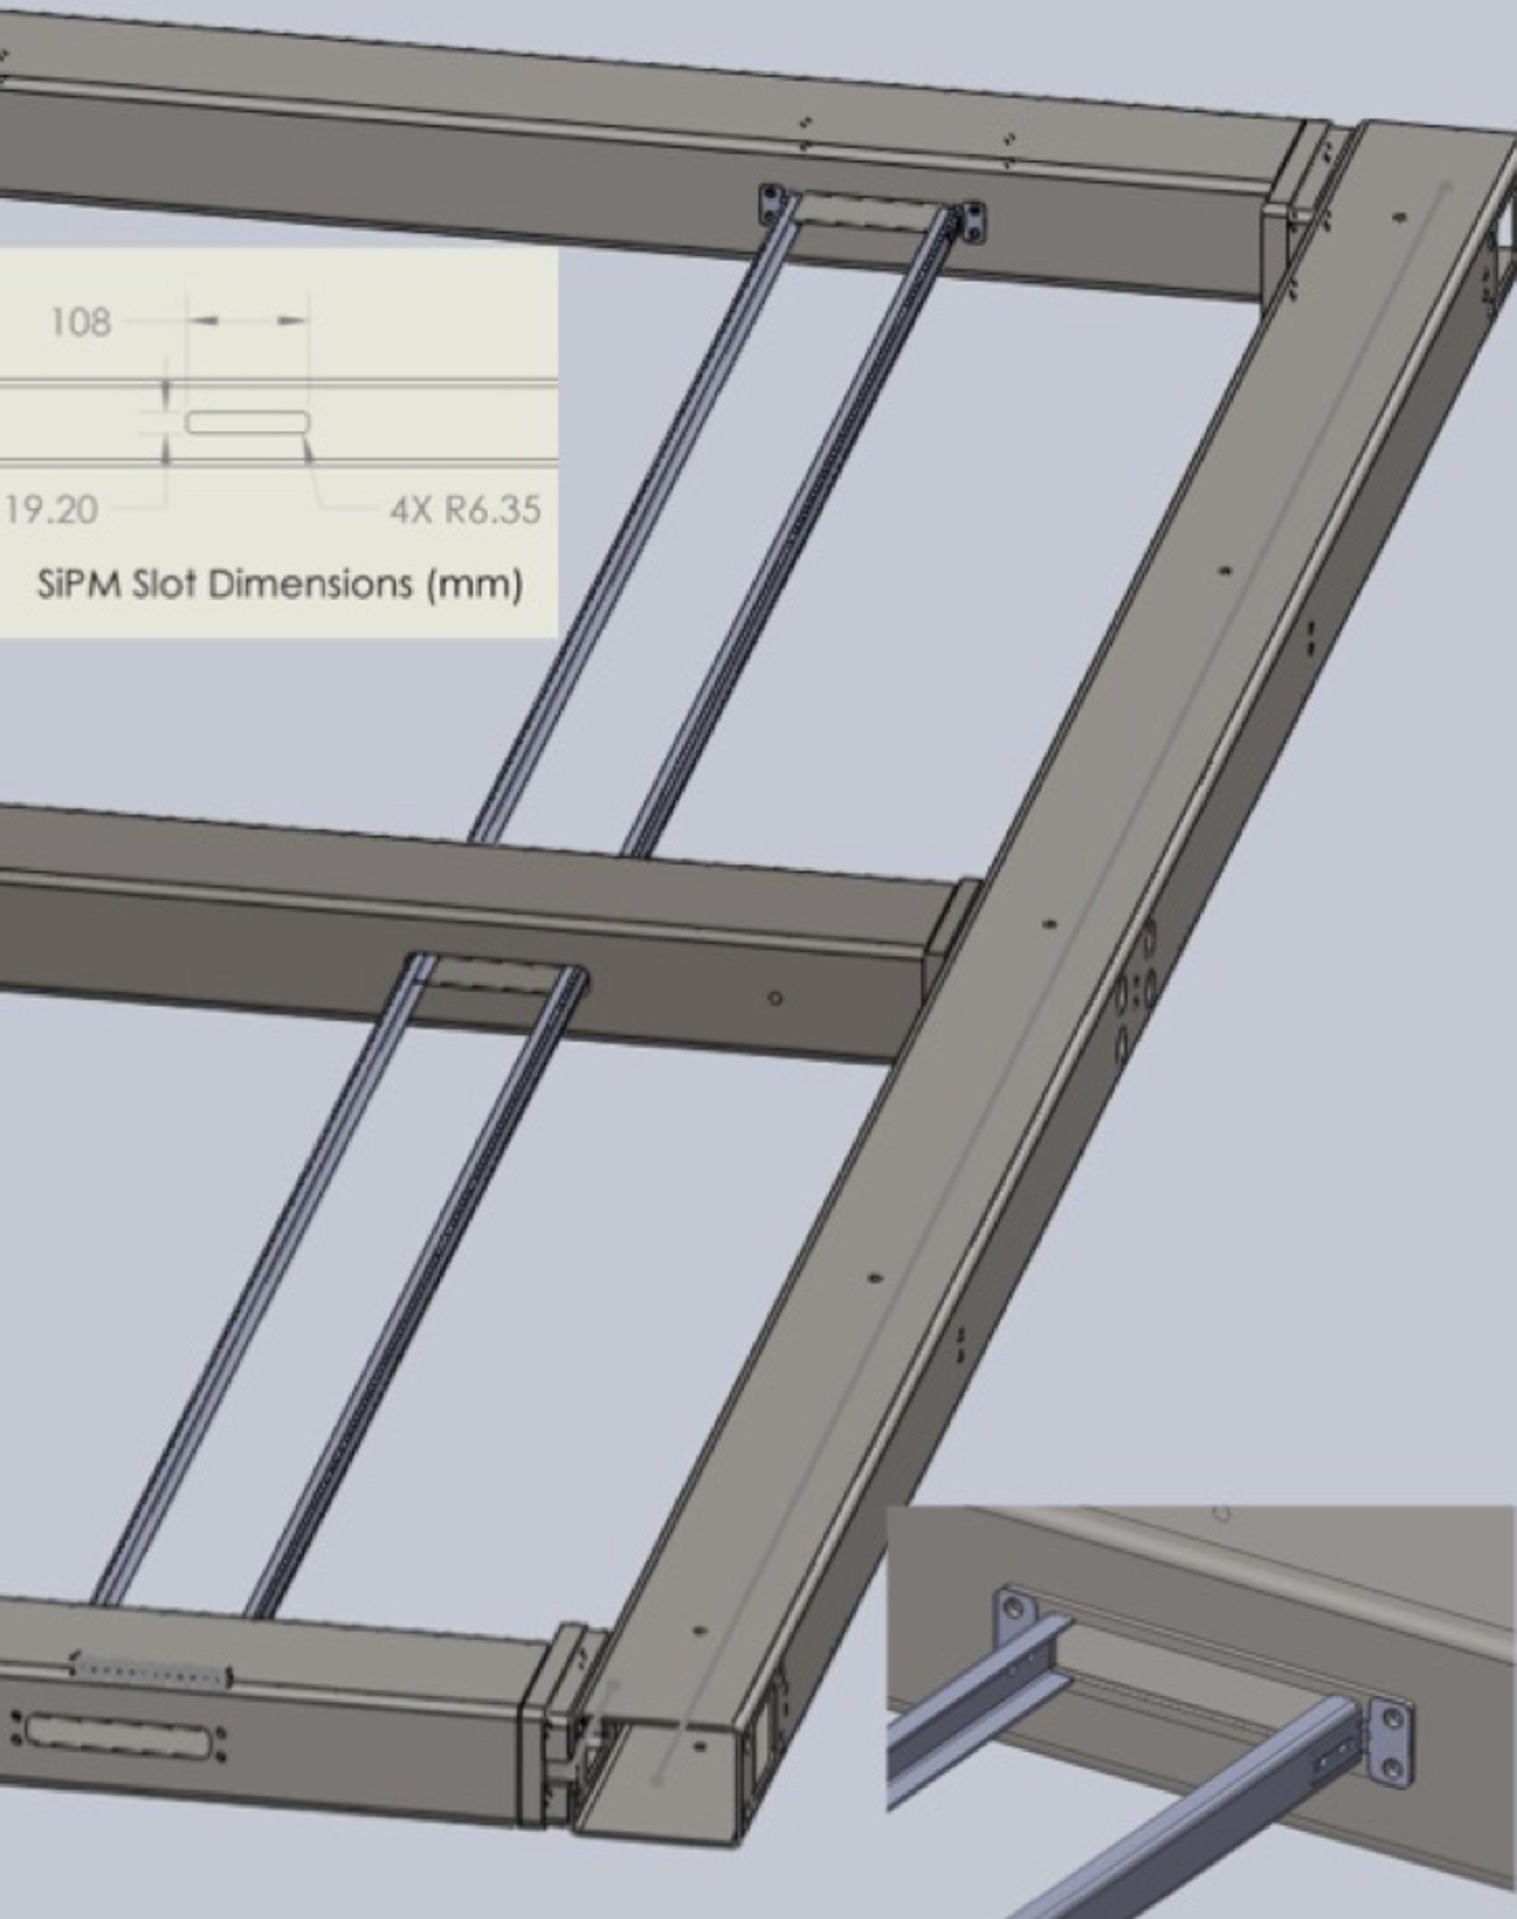
\includegraphics[height=7cm]{pds-pd-mounting-rails.pdf}
	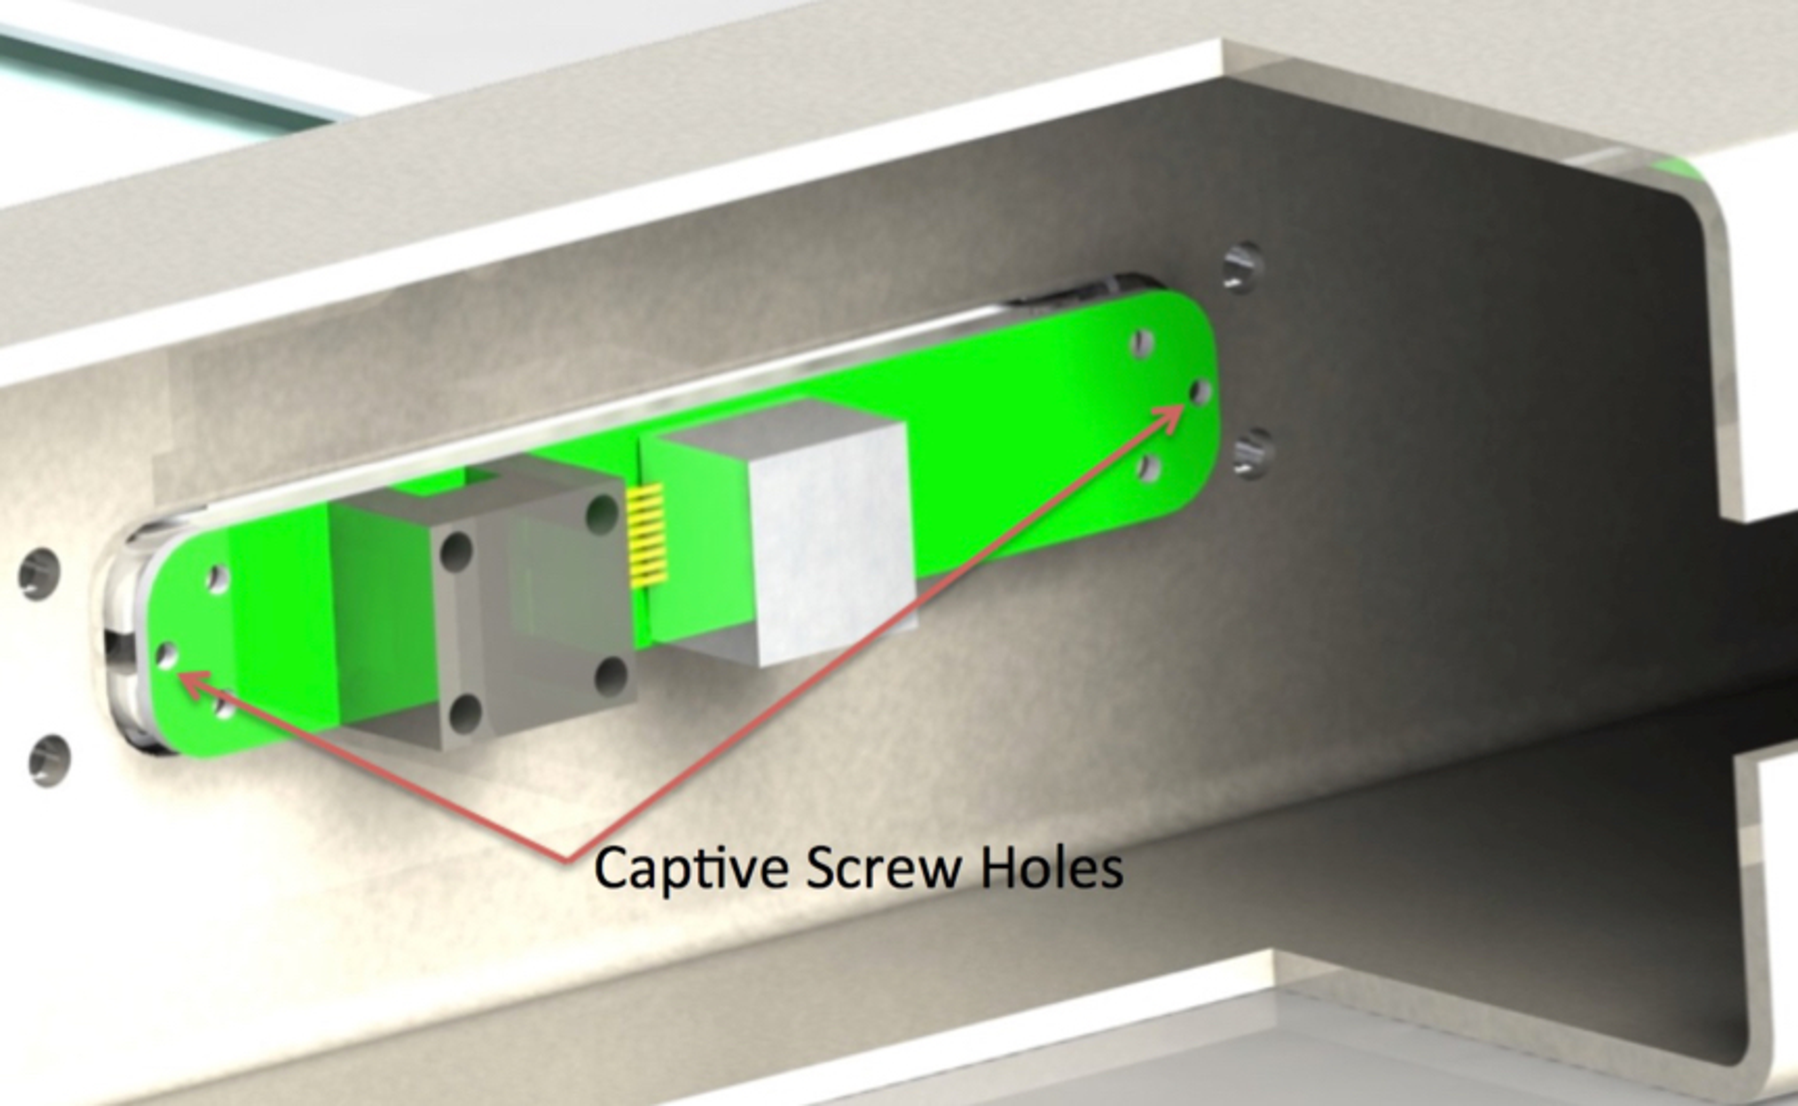
\includegraphics[height=5cm]{pds-pd-mounting-screws.pdf}
\end{dunefigure}


%\fixme{Insert Dave's PD Mounting screws mpicture}
%\begin{dunefigure}[Photon Detector mounting screws in APA frame.]{fig:pds-pd-mounting-screws}
%{Photon Detector mounting rails in APA frame.\fixme{alignment}}
%	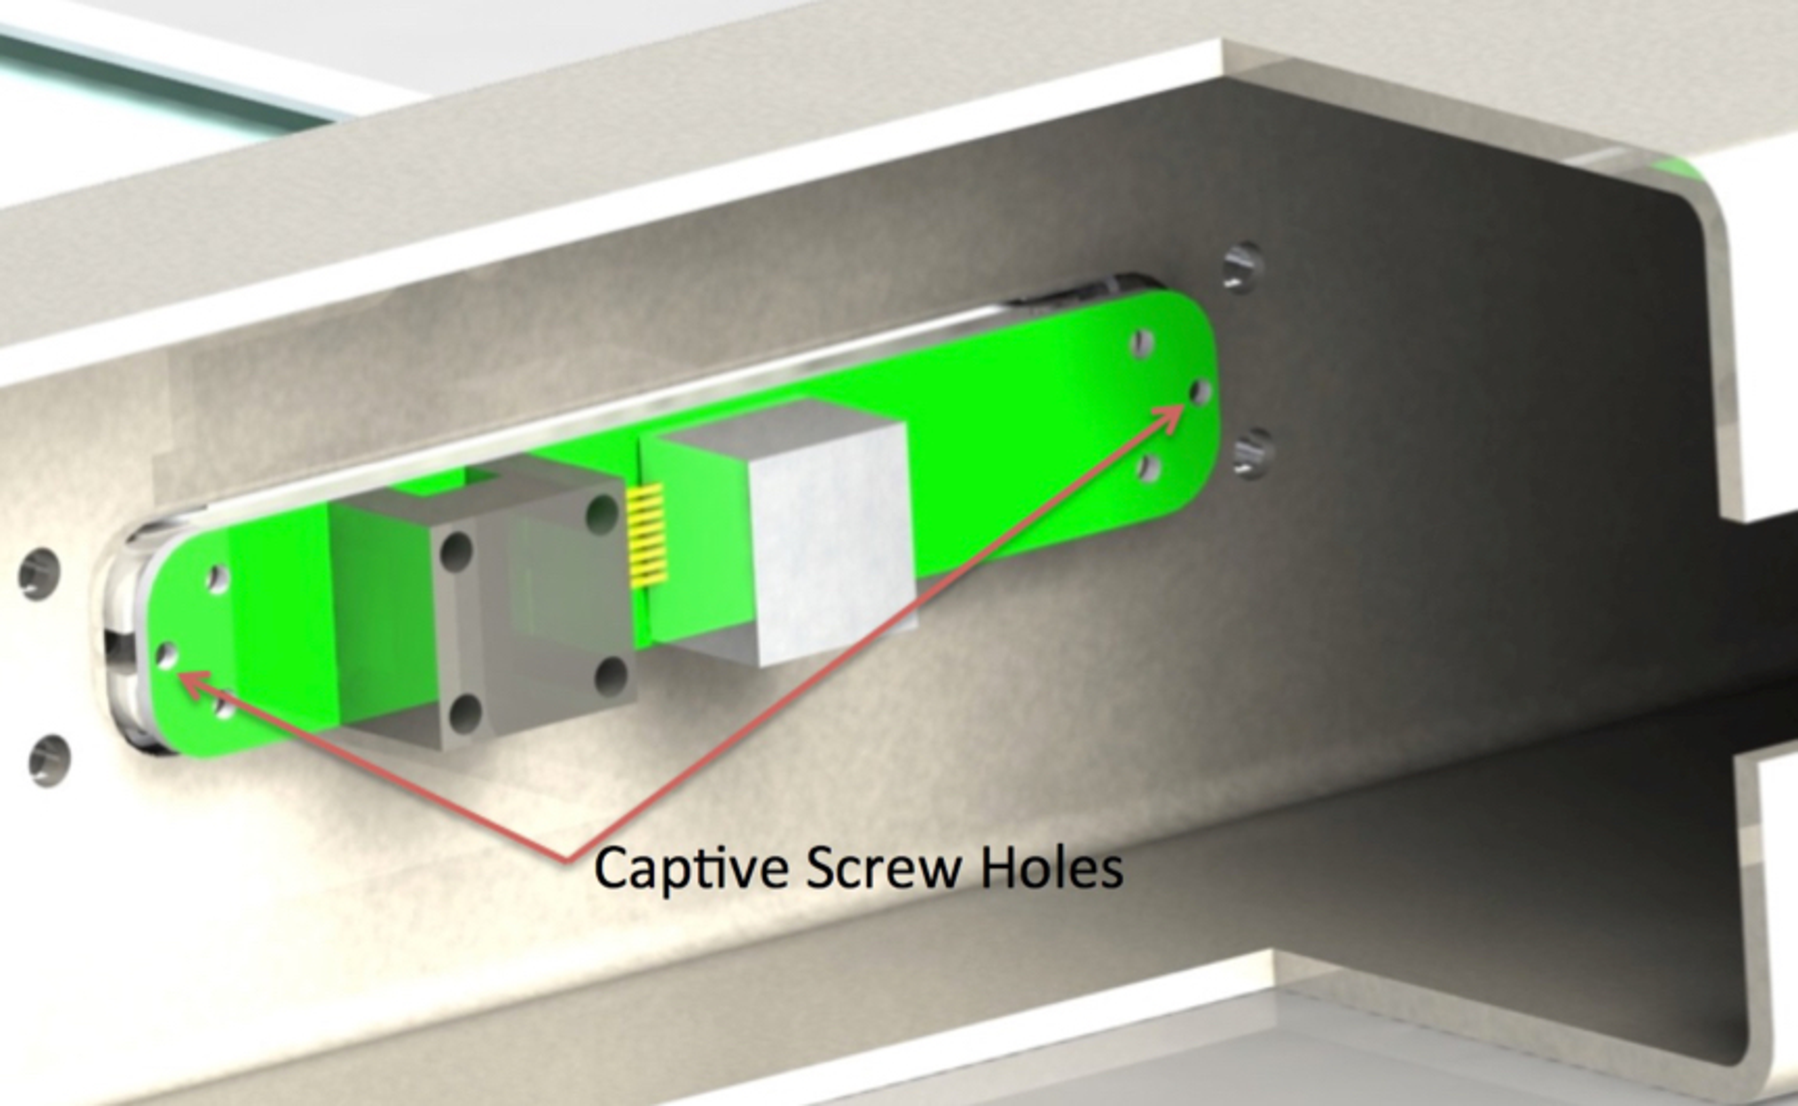
\includegraphics[height=5cm]{pds-pd-mounting-screws.pdf} 
%\end{dunefigure}


\subsubsection{Cryogenic thermal contraction}

Bar-style PD modules are structurally composed of primarily polycarbonate, polystyrene and 
acrylic, which have significantly different shrinkage factors compared to the 
stainless steel APA and PD support frames (see Table~\ref{tbl:fdsfpdshrink}).

\begin{dunetable}[Shrinkage of PD materials.]
%{|c|c|}
{cc}
{tbl:fdsfpdshrink}
{Shrinkage of PD module materials for a $206^{\circ}$C temperature drop}
Material 			 & Shrinkage Factor (m/m)\\ \toprowrule
Stainless Steel (304) & $2.7\times10^{-3}$\\ \colhline
FR-4 G-10 (In-plane) & $2.1\times10^{-3}$\\ \colhline
Polystyrene (Average) & $1.5\times10^{-2}$\\ \colhline
Acrylic and Polycarbonate (Average) & $1.4\times10^{-2}$\\ 
\end{dunetable}

These differences in thermal expansion (or contraction, in this case) are an important factor during design of the PD module supports.  Mitigation of these contractions is detailed in Table~\ref{tbl:fdsfpdshrinkeffects}.

Thermal expansion coefficients for the fused-silica filter plates ($1.1\times10^{-4}$~\si{m/m} for a 206$^\circ$C temperature drop) informed the materials selection for the ProtoDUNE ARAPUCA modules.  The frame components for the ARAPUCA were fabricated from FR-4 G-10, resulting in a shrinkage of the stainless steel frame structure relative to the frame of approximately \SI{1.2}{mm} along the long ($\sim$\SI{2}{m}) axis of the bar.  The shrinkage of the frame relative to the filter plate is <\SI{0.2}{mm}.  Both these relative shrinkage factors are accounted for in the dimensions and tolerances of the design.



\begin{dunetable}[Relative shrinkage of PD components and APA frame with mitigations]
%{|p{0.2\textwidth}|p{0.2\textwidth}|p{0.5\textwidth}l}
{p{0.2\textwidth}p{0.2\textwidth}p{0.5\textwidth}}
{tbl:fdsfpdshrinkeffects}
{Relative Shrinkage of PD components and APA frame, and mitigations}
\textbf{Interface} & \textbf{Relative shrinkage} & \textbf{Mitigation} \\ \toprowrule
PD Length to APA width & PD shrinks \SI{25.7}{mm} Relative to APA frame & PD affixed only at one end of APA frame, free to contract at other end \\ \colhline
Width of PD in APA Slot & PD shrinks \SI{1.2}{mm}  relative to slot width & Photon detector not constrained in C-channels. C channels and tolerances designed to contain module across thermal contraction range \\ \colhline
Width of SiPM mount board ({\it Hover board}) to stainless steel frame & Stainless frame shrinks \SI{0.06}{mm}  more than PCB & Diameter of shoulder screws and FR-4 board clearance holes selected to allow for motion \\ \colhline
Width of SiPM mount board relative to polycarbonate mount block & Polycarbonate block shrinks \SI{1}{mm} more than PCB & Allowed for in clearance holes in SiPM mount board \\ 
\end{dunetable}

\subsubsection{PD Mount frame deformation under static PD load}

FEA modeling of the PD support structure was conducted to study static deflection 
prior to building prototypes.  Modeling was conducted in both the vertical
 orientation (APA upright, as installed in cryostat) and also horizontal orientation.  
Basic assumptions used were fully-supported fixed end conditions for the rails, 
with uniform loading of 3X PD mass (\SI{5}{kg}) along rails.  
Figure~\ref{fig:pds-rail} illustrates the rail deflection for the APA in the horizontal (left) and vertical (right) orientations.
Prototype testing confirmed these calculations.

\begin{dunefigure}[PD mechanical support analysis.]{fig:pds-rail}
{PD mechanical support analysis: Rail deflection for the APA in the horizontal (left) and vertical (right) orientations.}
	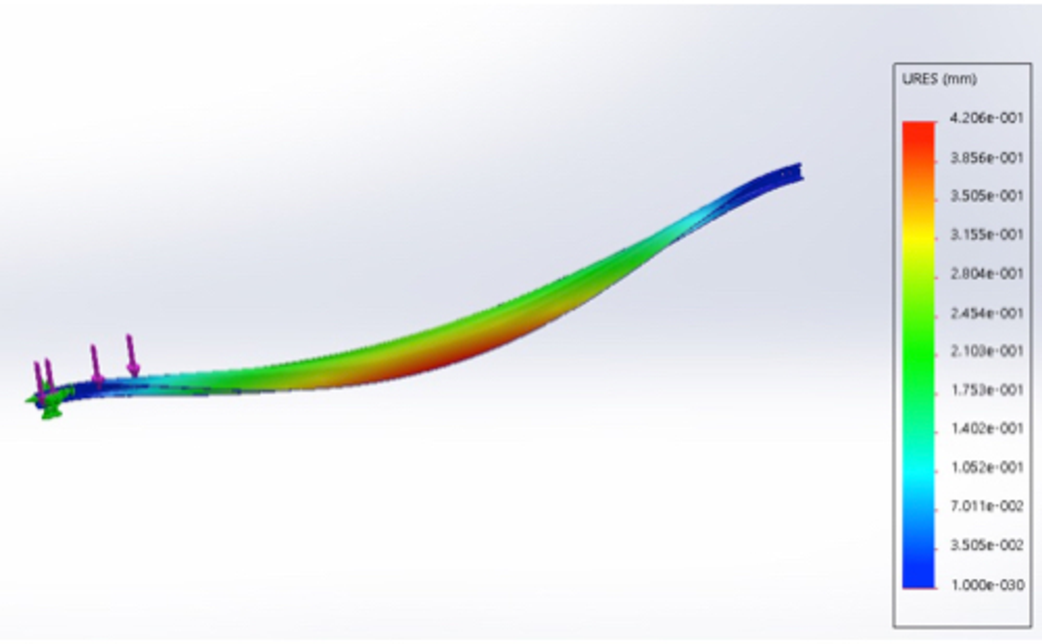
\includegraphics[height=4.5cm]{pds-rail-deflec-apa-flat.pdf} 
	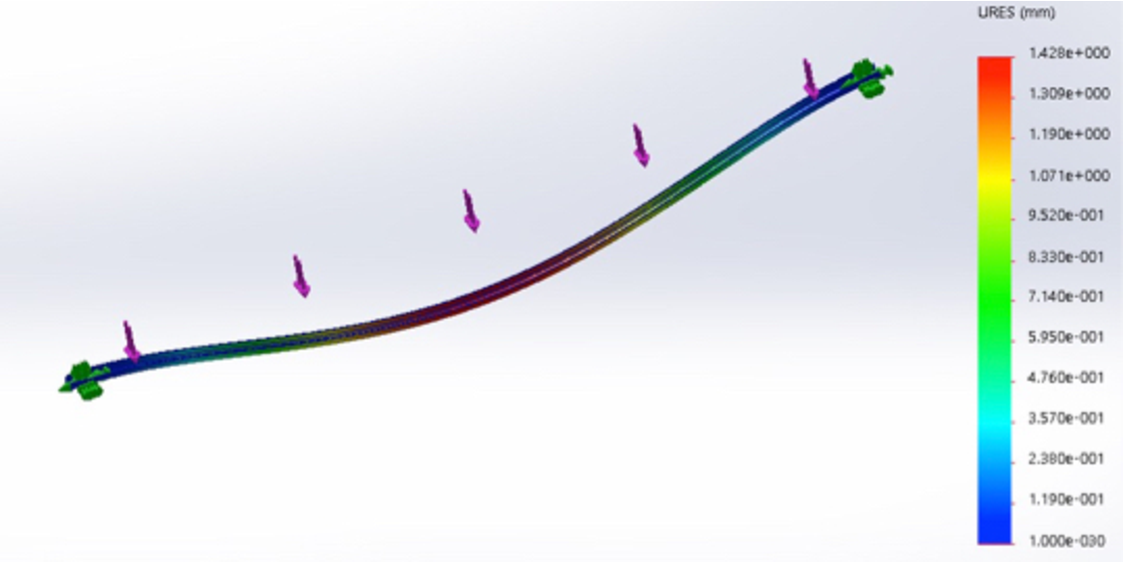
\includegraphics[height=4.5cm]{pds-rail-deflec-apa-vert.pdf}\\
%	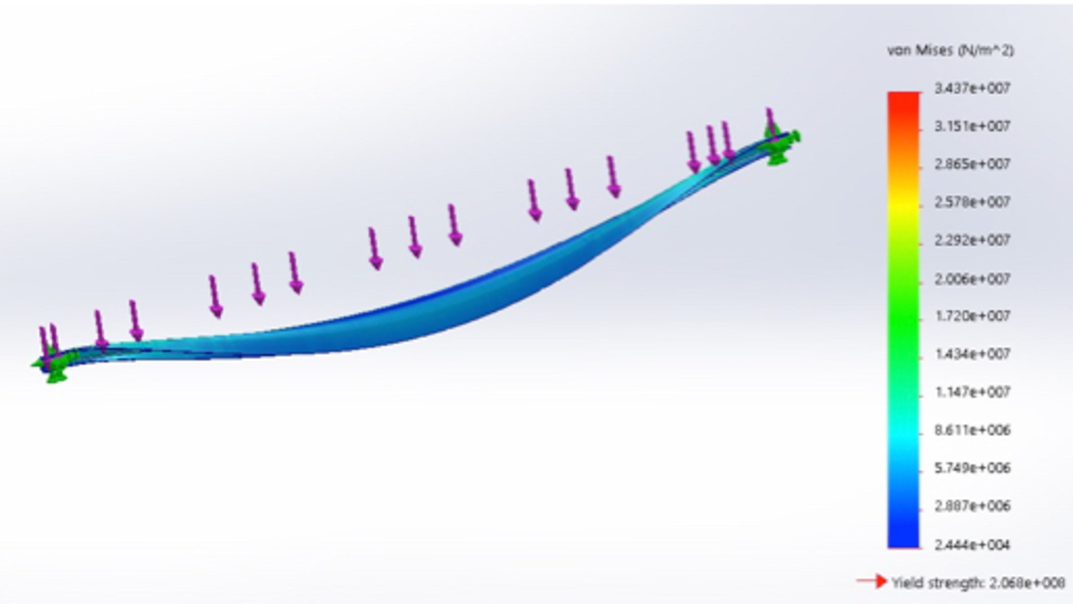
\includegraphics[width=0.25\columnwidth]{pds-rail-stress-apa-flat.pdf} 
%	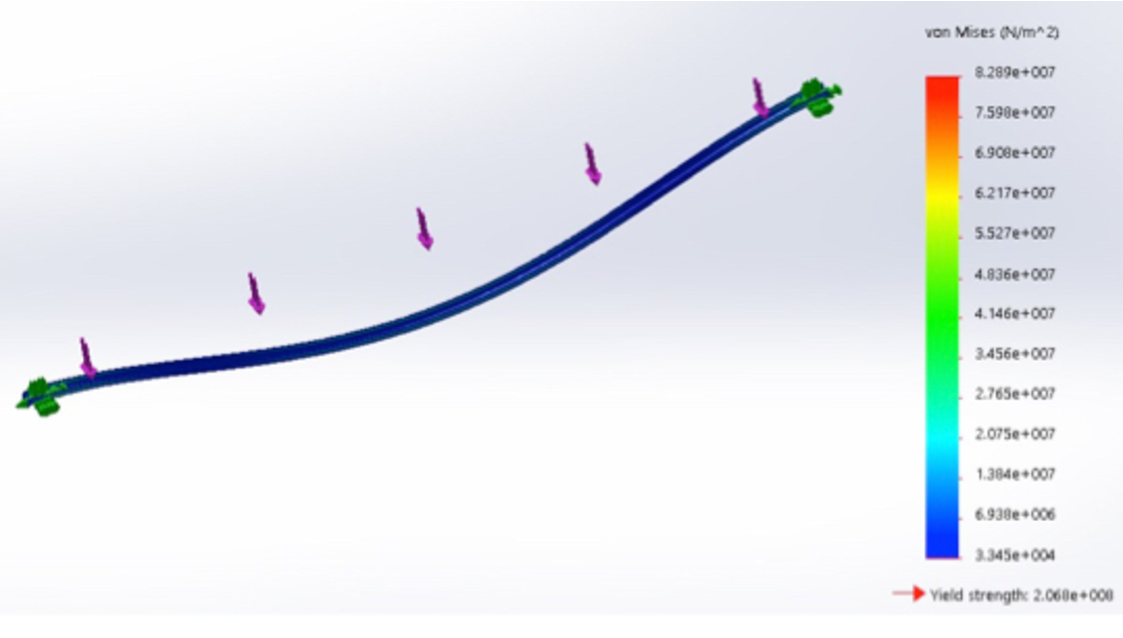
\includegraphics[width=0.25\columnwidth]{pds-rail-stress-apa-vert.pdf}
\end{dunefigure}


%%%%%%%%%%%%%%%%%%%%%%%%%%%%%%%%%%
\subsection{Photosensor Modules}
\label{sec:fdsp-pd-assy-psm}
%\todo{\color{blue} Content: Zutshi}

Depending on the photon collector  technology selected, the SiPM analog signal will be ganged in groups of 6-48 in close proximity to the sensors inside the
LAr volume; both {\it passive} and {\it active} ganging schemes are under consideration.  Passive ganging (sensors in parallel) implemented with traces on the SiPM mounting board (module) and has been implemented for ProtoDUNE-SP.  The SiPMs are mounted using a pick-and-place machine and standard surface mount device soldering procedures. 
 The ganged analog signals are then brought out via long cables (approximately \SI{25}{m}) for digitization outside the cryostat.
 ProtoDUNE-SP will provide essential operational experience with a passive ganging board and signal transport provided by Teflon ethernet CAT6 cables.
It is already apparent that R\&D is needed to optimize the connectors used to couple the cable to the board;  it is a priority to understand the 
mechanical stresses involved in the SiPM-PCB-Connector system (with different CTEs) as it is cooled (or cycled) to cryogenic temperatures.
 
A basic level of active ganging locates summing circuitry on the board carrying the photosensors or on a separate PCB also mounted on the PD module.
A more complex scheme is being considered that would include cold amplifiers and ADCs. This solution would provide more flexibility in the level of photosensor ganging and also obviate the need for carrying analog signals of long cables. Production of the board would follow standards practices but the complexity introduces concerns with reliability and long-term stability issues related to cold electronics.  Basic active ganging prototypes are under study with high priority but the design is not yet at a mature stage. 

%Schedule, cost and other technical considerations will influence how far this promising option can be pursued.
%%Moved to the Design section%%The terminal capacitance of the sensors strongly affects the signal-to-noise when devices are ganged in parallel and so is a factor in SiPM selection, and may ultimately determine  the maximum number of individual sensors that can be ganged this way. 

%In all scenarios considered, the SiPMs will be surface-mounted on a PCB that can mate efficiently with the photon collector options. 


%%%%%%%%%%%%%%%%%%%%%%%%%%%%%%%%%%
\subsection{Electronics}
\label{sec:fdsp-pd-assy-pde}
%\metainfo{\color{red}  Content: (2 pages) Moreno/Franchi/Djurcic}
%\todo{\color{blue}  Content: Moreno/Franchi/Djurcic}

Extensive experience of manufacturing processes was gained during the development of the SSPs under current use on ProtoDUNE-SP, a general description of the readout system of ProtoDUNE-SP can be seen in the section \ref{sec:fdsp-pd-pde}. Compatibility between elements designed by different institutions is guaranteed when standard procedures are followed so the circuit design must be done in accordance with mutually agreed-upon specification documents.  A sufficient  number of units needs to be produced to allow local testing and for testing in the central facility - for example, in ProtoDUNE-SP \num{5} 12-channel  SSPs were produced and delivered to CERN for integration testing prior. Twenty-four were fabricated for ProtoDUNE operation. 

The readout electronics of the photon detection system will be designed and produced with similar tools and protocols used for  ProtoDUNE-SP. For example: printed circuit board (PCB) layout is performed in accordance with IPC specifications. Bare PCB manufacturing requirements are embedded within the Gerber file fabrication documents (e.g. layers, spacing, impedance, finish, testing, etc.). Components are assembled on to circuit boards using either trained PD consortium technical staff or by external assembly vendors, based upon volume, in accordance with per-design assembly specification documents. Testing occurs at labs and universities within the collaboration in accordance with a per-design test procedure that typically includes a mix of manual, semi-automatic and automated testing in an engineering test bench followed by overall characterization in a system- or subsystem-test stand.
Other considerations and practices relevant to readout electronics production and assembly are itemized here:

\begin{itemize}

\item Components: Schematic capture is done using appropriate tools (such as OrCAD 16.6.\footnote{OrCAD\texttrademark{} schematic design tool for PCB design http://www.orcad.com} or similar toolset) available within design facility. Design is hierarchical with common front-end page referenced multiple times to ensure that all input channels are identical. The schematic contains complete bill-of-materials (BOM) including all mechanical parts. Subversion repository is typically used for version control and backup. Multiple internal design reviews held before schematic is released to layout. The bill of materials is stored directly within schematic, extracted to spreadsheet when ordering parts. Every part is specified by both manufacturer and distributor information. Distributor information may be overridden by a technician at order time due to price and/or availability. Standard search engines such as Octopart\footnote{Octopart https://octopart.com/}, ECIA\footnote{ ECIA https://www.eciaauthorized.com} and PartMiner\footnote{PartMiner https://www.part-miner.com/} are used to check price/availability across all standard distributors. A parts availability check review is performed prior to handoff from schematic to layout; as required obsolete or long lead time parts were removed from design and replaced. BOM information will include dielectric, tolerance, temperature coefficient, voltage rating and size (footprint) to ensure all parts are fully described.

\item Boards: There are standard tools (such as the Allegro\footnote{Cadence Allegro\textregistered PCB design solution https://www.cadence.com} toolset) available for the printed-circuit-board (PCB) layout. Conventional PCBs are realized as multi-layer, controlled impedance board with many sets of delay-matched nets. In usual practice the complete impedance and delay characteristics are calculated within layout tool and crosschecked by PCB vendor prior to manufacture. In usual practice, a competitive bid between multiple previously qualified vendors is used, with a full electrical and impedance testing required. Multiple internal design reviews are held prior to release of the design.

\item Cable plant: Cabling will be designed taking into consideration the APA space and in close collaboration with the TPC electronics group to avoid cross-talk effects. A final decision on cable procurement will be taken based on the possibility of cable manufacturing in an institution belonging to the photon detection consortium and the cost of a commercial solution.  

\item Manufacturer list: In addition to the general laboratory procedures for quality assurance, the general practice will be to use only printed circuit board manufacturers and external assembly vendors whose workmanship and facilities have been personally inspected by experienced production team members. All external assemblers are required to quote in accordance with an Assembly Specification document describing the IPC class and specific solder chemistry requirements of the design. The Bill of Materials document will show selected and alternate suppliers for every component of the front-end boards.

\item Front-end electronics firmware: This will be specified and updated iteratively in collaboration with other systems. The electronics working group will be responsible for responding to requests for additional firmware development, including for example, modifications to timing interface, modifications to trigger interface, and implemented sensitivity to in-spill vs. not-in-spill conditions. Documents describing firmware architecture for each major change will be written and distributed to photon detector and DAQ working groups before implementation. Front-End electronics User's manual containing all details of new firmware will be distributed with production units when manufactured.

\item Mechanical assembly: With the mechanical assembly of electronics readout boards it is common practice to use AutoCAD\footnote{AutoDESK AutoCAD\textregistered computer aided design software application https://www.autodesk.com/} with Allegro (as PCB layout tool). All relevant dimensions of the PC board including connector and indicator placement is extracted from Allegro as base DXF file from which overall exploded mechanical diagram of chassis and other mechanical parts is made. Mechanical items such as shield plates will be provided as well. It is assumed that the front-end chassis will made by external vendors (one for chassis, one for front/back panels) from AutoCAD drawings provided by the consortium.

\end{itemize}
